\documentclass{article}
\usepackage{geometry, graphicx, float, subfigure, amsmath, bm, threeparttable,multirow, multicol, pgffor,ifthen}
\usepackage[justification=centering]{caption}
\usepackage[marginal]{footmisc}
\geometry{a4paper,scale=0.8}
\setlength{\parindent}{2em}

\title{\bf{The Analysis of Probabilities of Conjugation between E.coli and Transposition Mutagenesis of }$kan^R$}
\author{Xun Zhao (Partner: Chase)}
\date{April 19, 2019}

\begin{document}
    \begin{titlepage}
        \maketitle
        \setcounter{page}{0}
        \thispagestyle{empty}
    \end{titlepage}

    \renewcommand{\abstractname}{Introduction}
    \begin{abstract}
		The "jumping" gene was dicovered by McClintock who found spots on corn with different colors. Later, it was found that this phenomenon also happens in other species. 
		
		Conjugation is a cell-to-cell contact that can transfer plasmid and the genes on this plasmid from one bacteria cell to another, through a mating bridge called pilus. Transposon is a part of DNA sequence that can move or duplicate itself from one place to another even to different chromosomes. When the transposon is inserted into a gene, it can knock out the old gene and replace its function with new gene's function, which is called transposition mutagenesis.

		The first part of this experiment is to mate two strains of \emph{E.coli}, and let conjugation happens. The second part is using IPTG to induce $kan^R$ transposon on the plasmid to transpose.

		If conjugation happens, the recipient cell will get the $cm^R$ gene from pVJT128 plasmid, becoming insensitive to chloramphenicol. If transposition happens, the cell will have functional $kan^R$ gene, and become insensitive to kanamycin. If transposition mutagenesis happens at the \emph{lacZ} gene, the colony will be white on X-gel plates, due to it does not have the functional enzyme to digest X-gel.
	\end{abstract}

	\section{Results}
		\subsection{Conjugation}
			\begin{table}[H]
				\caption{Conjugation Data}
				\centering
				\begin{tabular}{|c|c|c|c|c|c|}
					\hline
					Mating Tube&Dilution&$10^0$&$10^{-1}$&$10^{-2}$&$10^{-3}$\\\cline{2-6}
					Cm-Nal Plates&\#Colonies&508&2&0&0\\\hline
					Recipient Tube&Dilution&$10^{-5}$&$10^{-6}$&$10^{-7}$\\\cline{2-5}
					NA Plates&\#Colonies&946&107&13\\\cline{1-5}
					Recipient Tube&Dilution&$10^0$\\\cline{2-3}
					Cm Plates&\#Colonies&135\\\cline{1-3}
					Donor Tube&Dilution&$10^0$\\\cline{2-3}
					Nal Plates&\#Colonies&0\\\cline{1-3}
				\end{tabular}
				\label{conjugation.data}
			\end{table}
		\subsection{Percent Conjugation}
			$$
			\begin{aligned}
			\text{Conjugation}\% &= \frac{\#\text{Cm.Nal} - \#\text{Reversion.Recipient} - \#\text{Reversion.Donor}}{\#\text{NA.Total}}\\
			&= \frac{508 - 135- 0}{\frac{946 + 107 \times 10 + 13 \times 100}{3} \times 10 ^{5}}\\
			&= \frac{373}{1105 \times 10 ^ 5}\times 100\%\\
			&\approx 3.4 \times 10 ^ {-4}\%
			\end{aligned}
			$$
		\subsection{Transposition and Mutagenesis}
			\begin{table}[H]
				\caption{Transposition and Mutagenesis Data}
				\centering
				\begin{tabular}{|c|c|c|c|c|c|c|}
				\hline
				\multirow{3}*{\shortstack{Inducing Tube\\X-gel Kan Plates}}&\multicolumn{2}{|c|}{Dilution}&$10^0$&$10^{-1}$&$10^{-2}$&$10^{-3}$\\\cline{2-7}
				~&\multirow{2}*{\#Colonies}&White&-&3&0&0\\\cline{3-7}
				~&~&Blue&-&8654&728&94\\\hline
				Inducing Tube&\multicolumn{2}{|c|}{Dilution}&$10^{-4}$&$10^{-5}$&$10^{-6}$&$10^{-7}$\\\cline{2-7}
				NA Plates&\multicolumn{2}{|c|}{\#Colonies}&-&820&103&12\\\hline
				\end{tabular}
				\label{transposition.mutagenesis.data}
			\end{table}
		\subsection{Percent Transposition}
			$$
			\begin{aligned}
			\text{Transposition}\% &= \frac{\#\text{X-gel.Kan}}{\#\text{NA.Total}}\\
			&= \frac{((8654 + 3) + 728 \times 10 + 94 \times 100) / 3}{((103 \times 10 + 12 \times 100) / 2) \times 10 ^4}\\
			&= \frac{8445}{1115 \times 10 ^4} \times 100\%\\
			&\approx 0.076\%
			\end{aligned}
			$$
		\subsection{Percent Mutagenesis}
			$$
			\begin{aligned}
			\text{Mutagenesis}\% &= \frac{\#\text{X-gel.Kan.White}}{\#\text{X-gel.Kan.Total}}\\
			&= \frac{3}{((8654 + 3) + 728 \times 10 + 94 \times 100) / 3}\\
			&= \frac{3}{8445} \times 100\%\\
			&\approx 0.35\%
			\end{aligned}
			$$
	\section{Discussion}
		\subsection{Conjugation}
			\begin{figure}[H]
				\begin{minipage}[t]{0.24\textwidth}
					\centering
					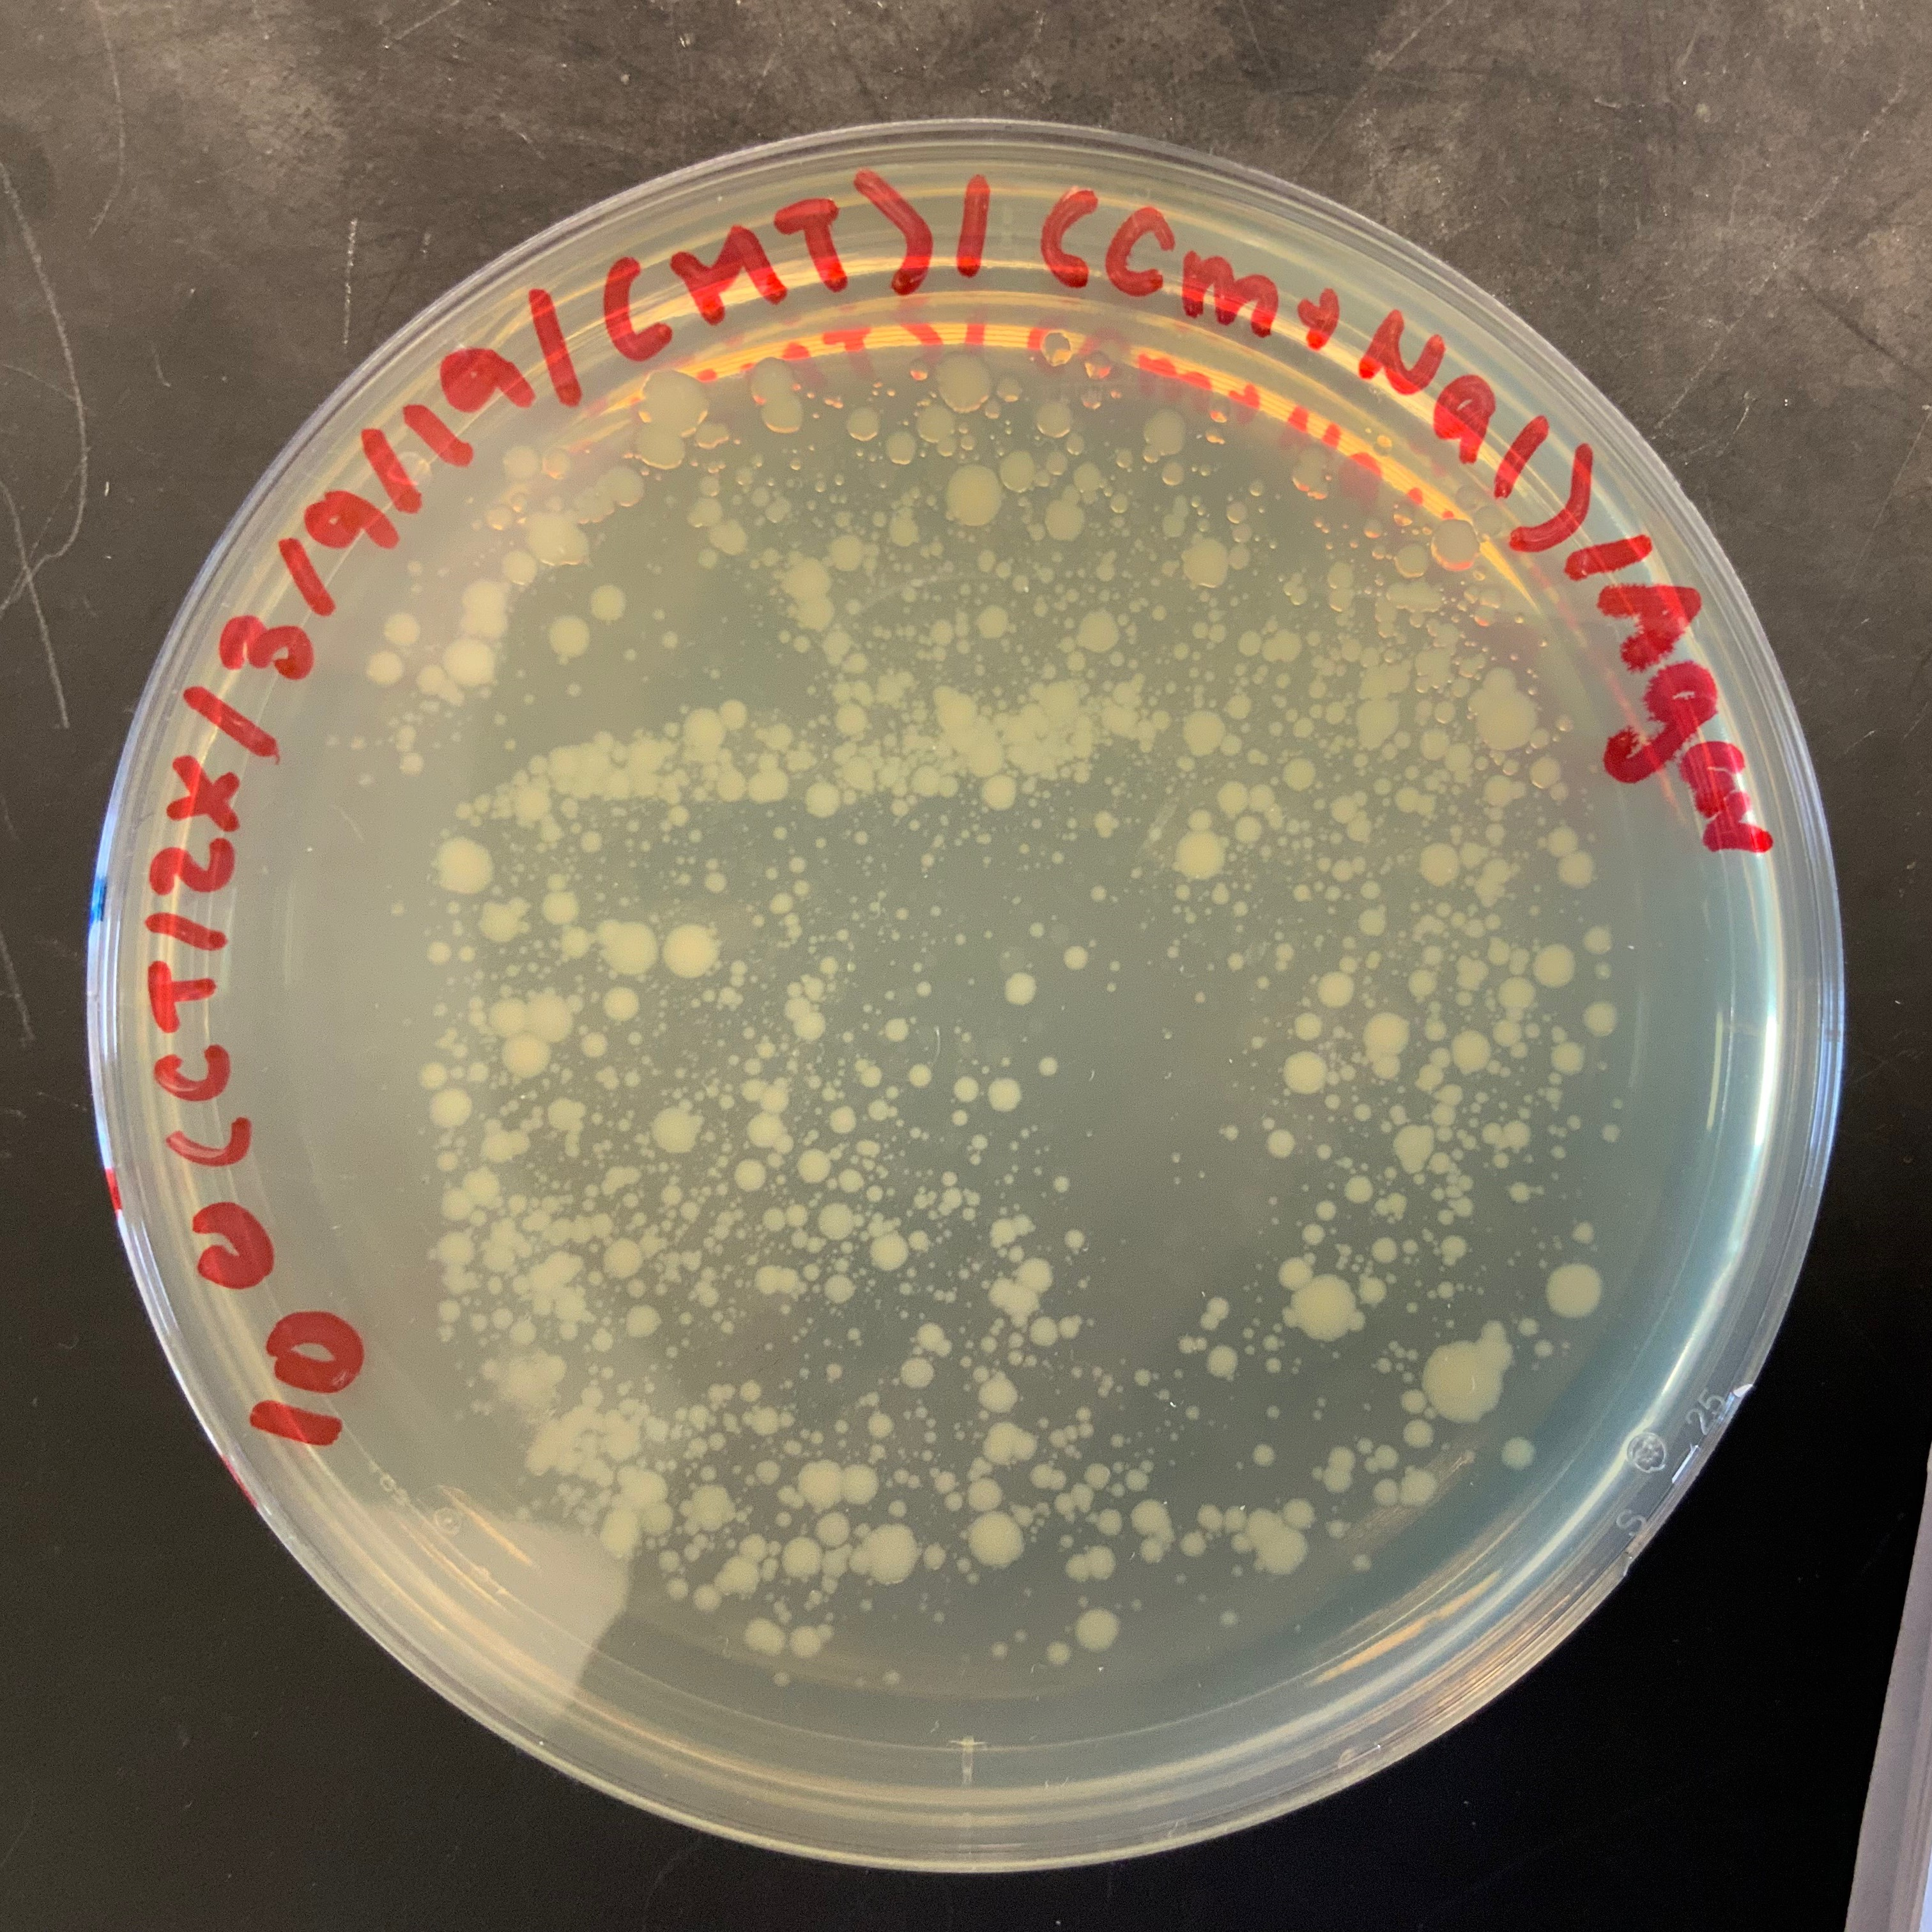
\includegraphics[width = 0.9\linewidth]{Mate_0_NalCm.jpg}
					\captionsetup{font={scriptsize}}\caption{MT $10^{0}$ Cm-Nal, 508}
				\end{minipage}
				\begin{minipage}[t]{0.24\textwidth}
					\centering
					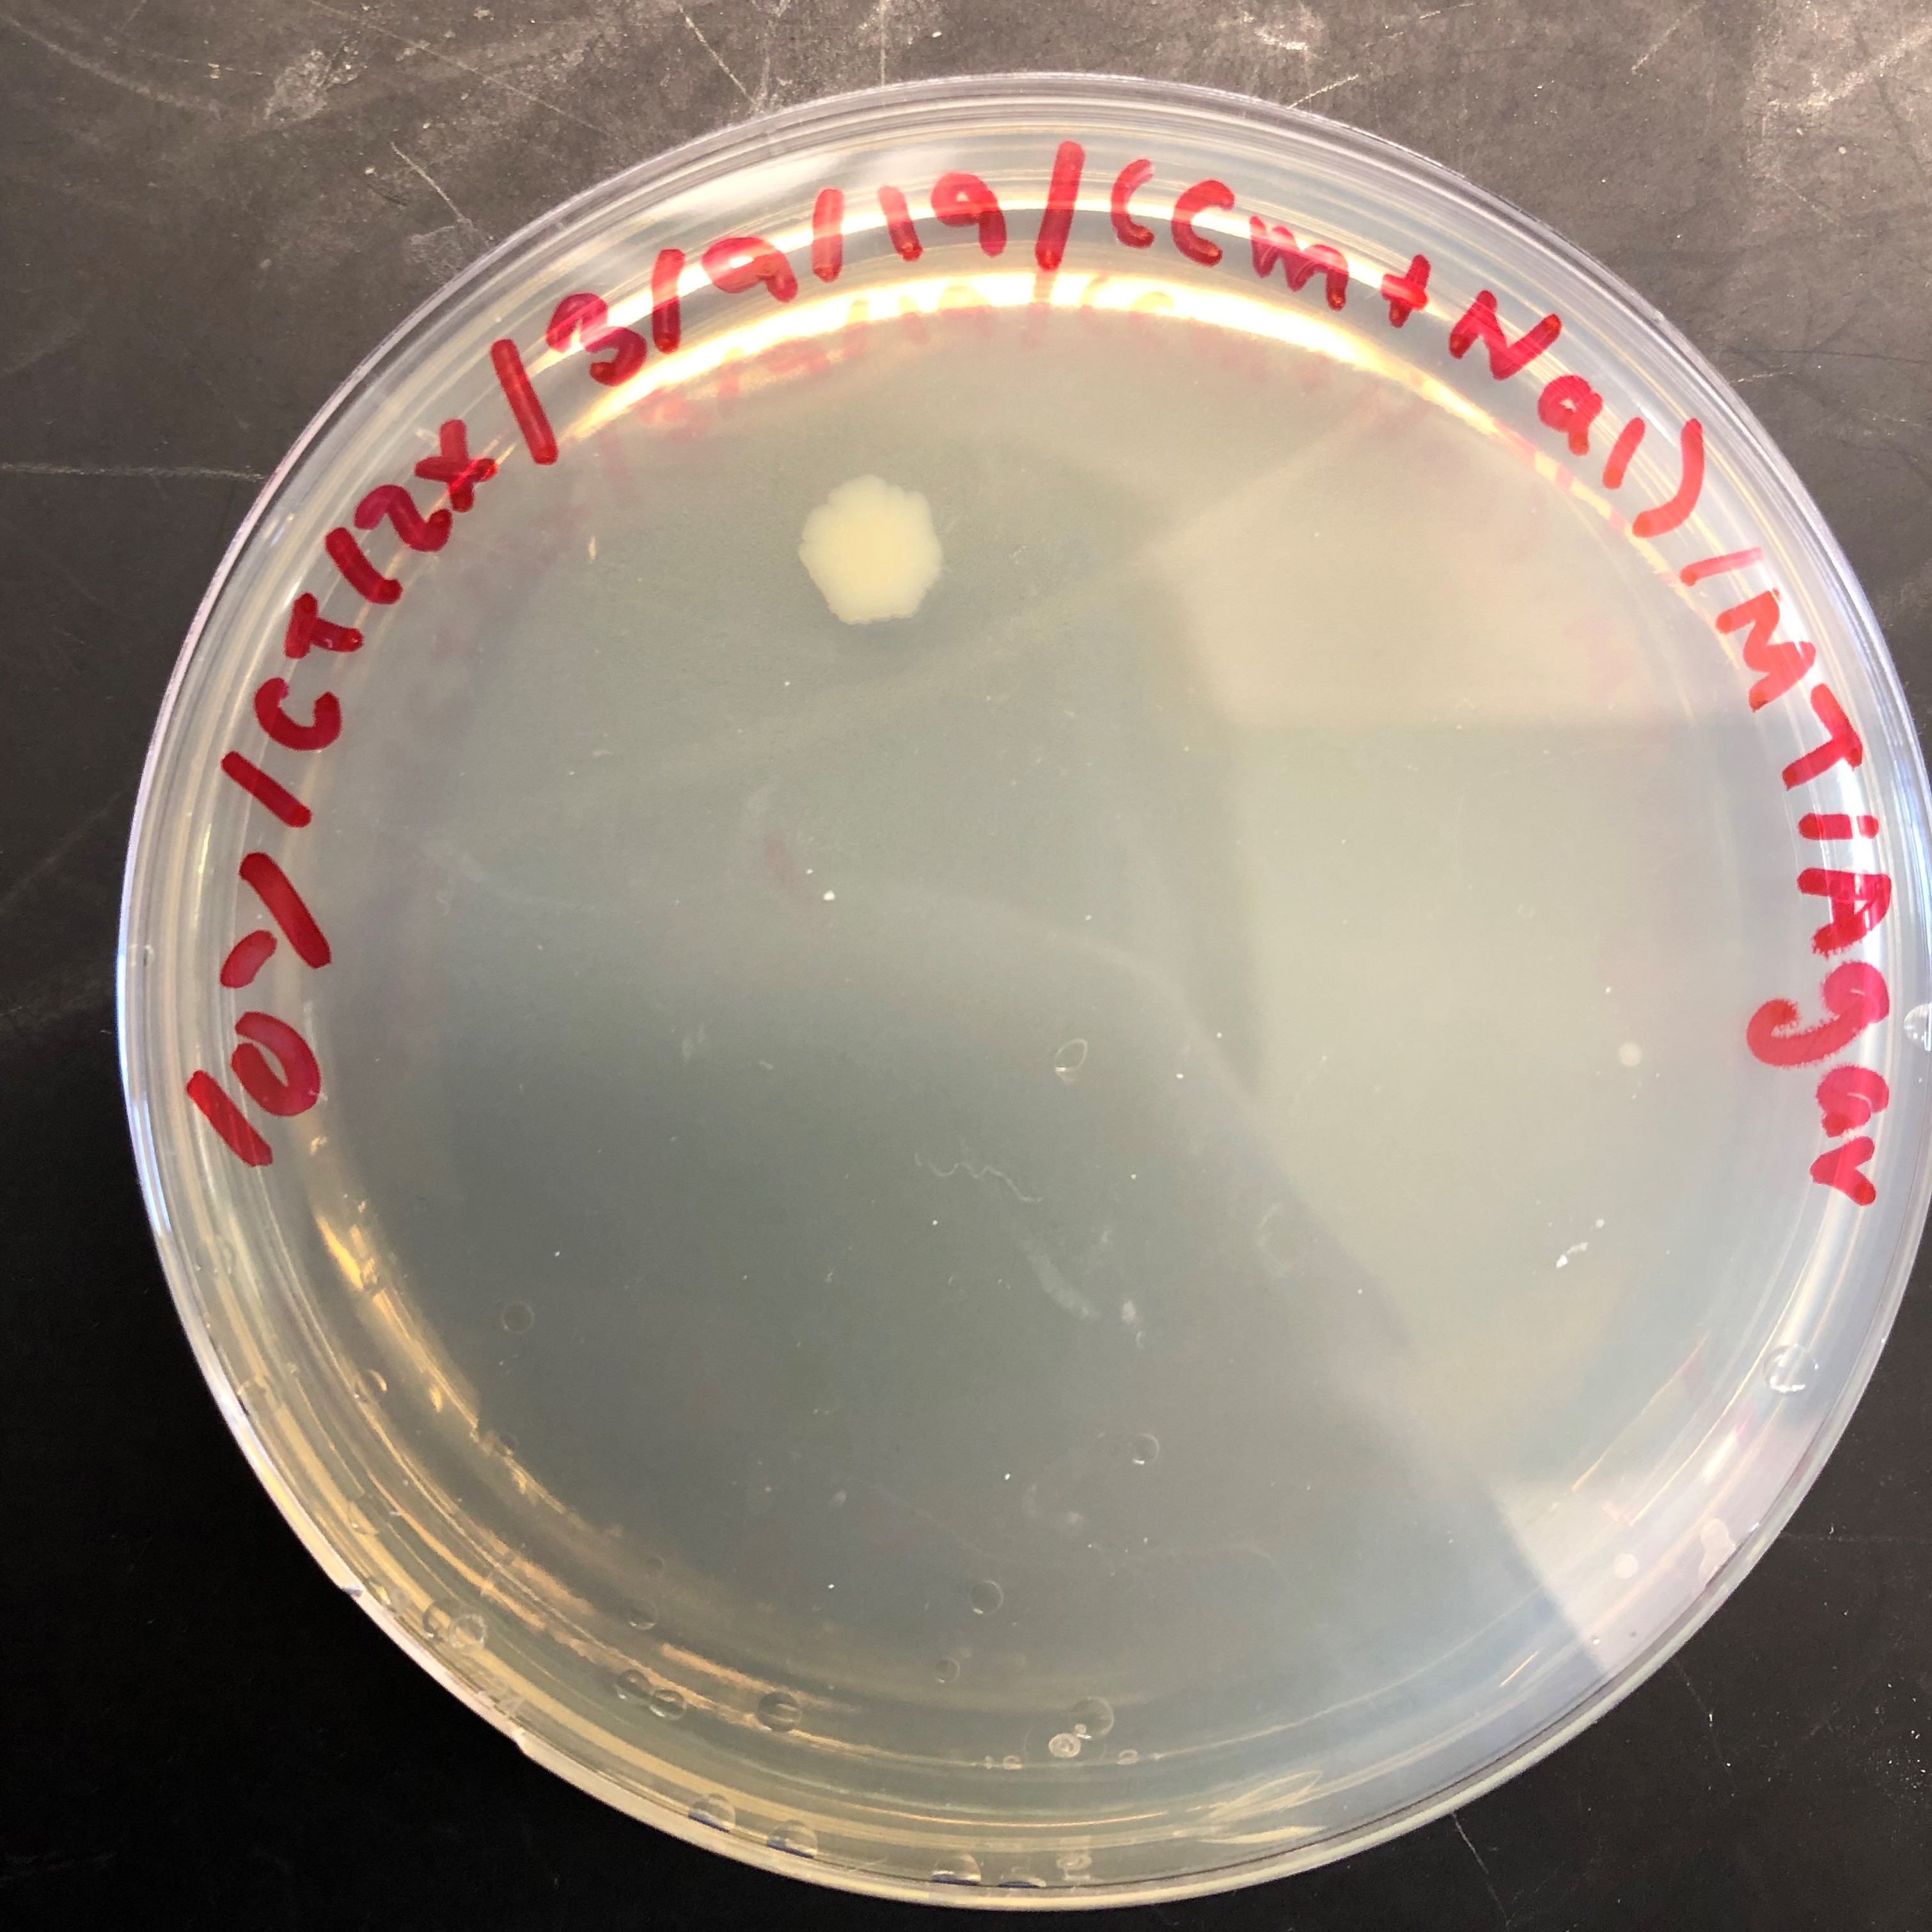
\includegraphics[width = 0.9\linewidth]{Mate_1_NalCm.jpg}
					\captionsetup{font={scriptsize}}\caption{MT $10^{-1}$ Cm-Nal, 2}
				\end{minipage}
				\begin{minipage}[t]{0.24\textwidth}
					\centering
					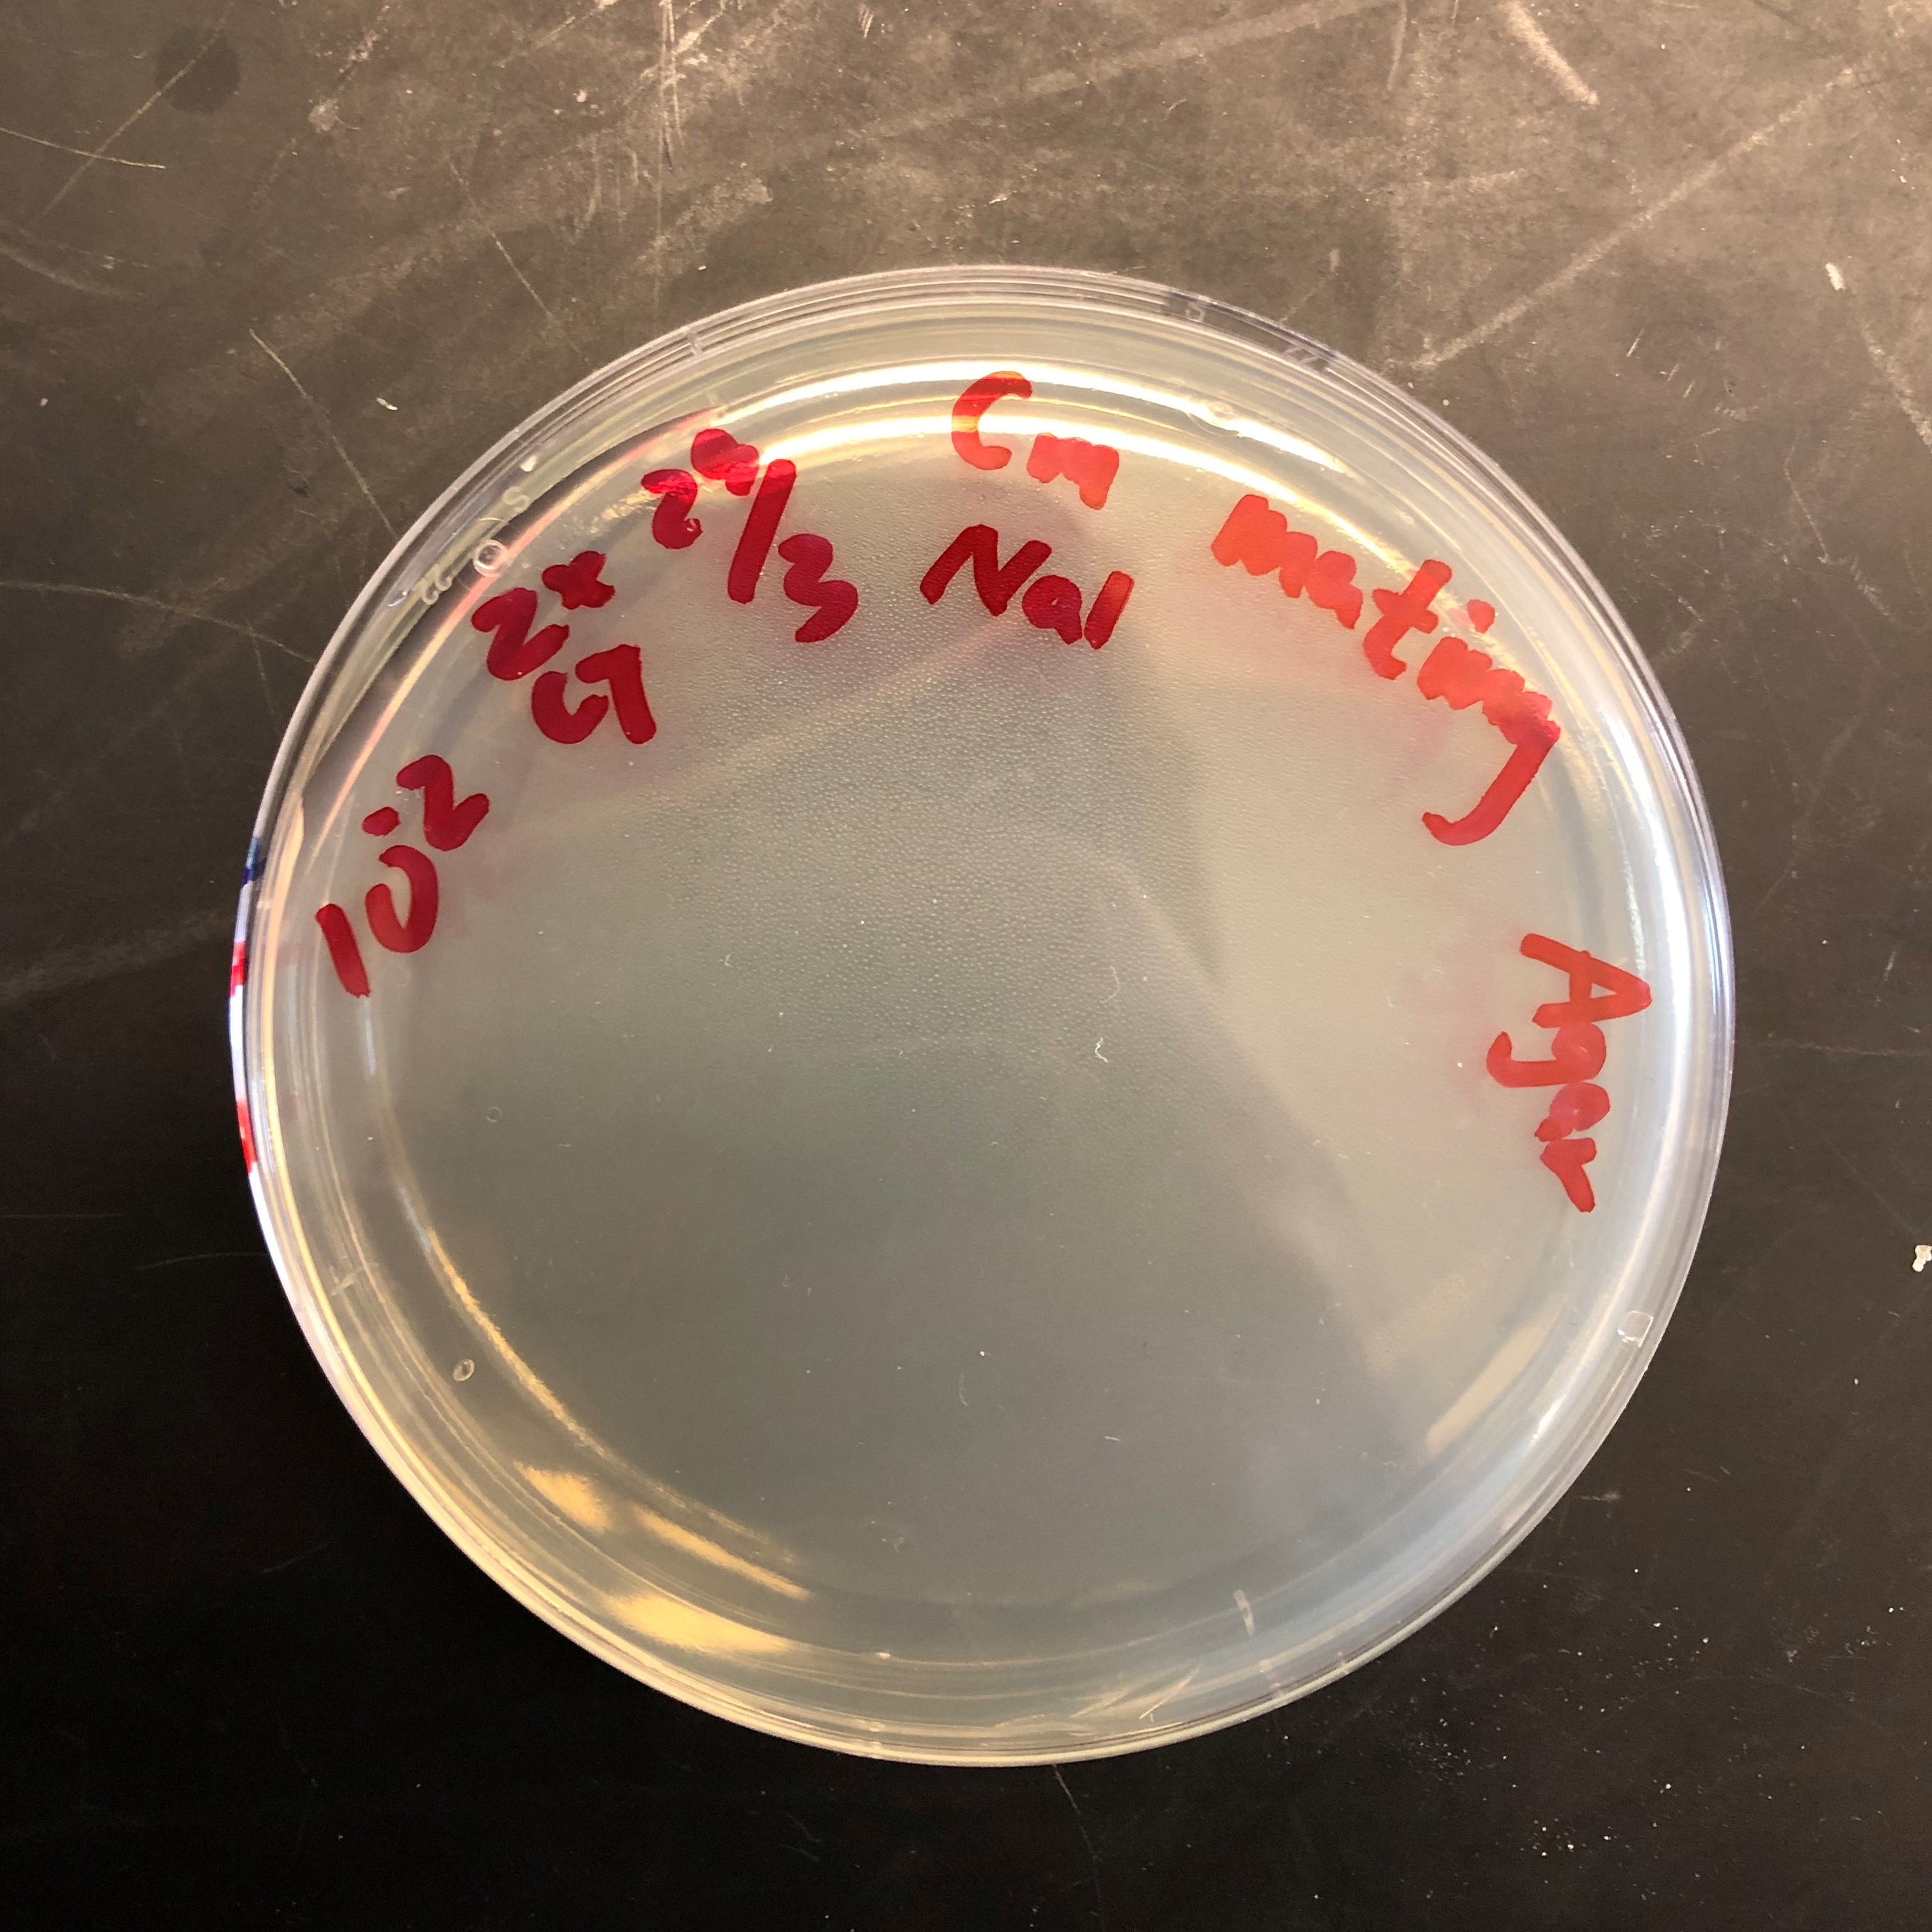
\includegraphics[width = 0.9\linewidth]{Mate_2_NalCm.jpg}
					\captionsetup{font={scriptsize}}\caption{MT $10 ^ {-2}$ Cm-Nal, 0}
				\end{minipage}
				\begin{minipage}[t]{0.24\textwidth}
					\centering
					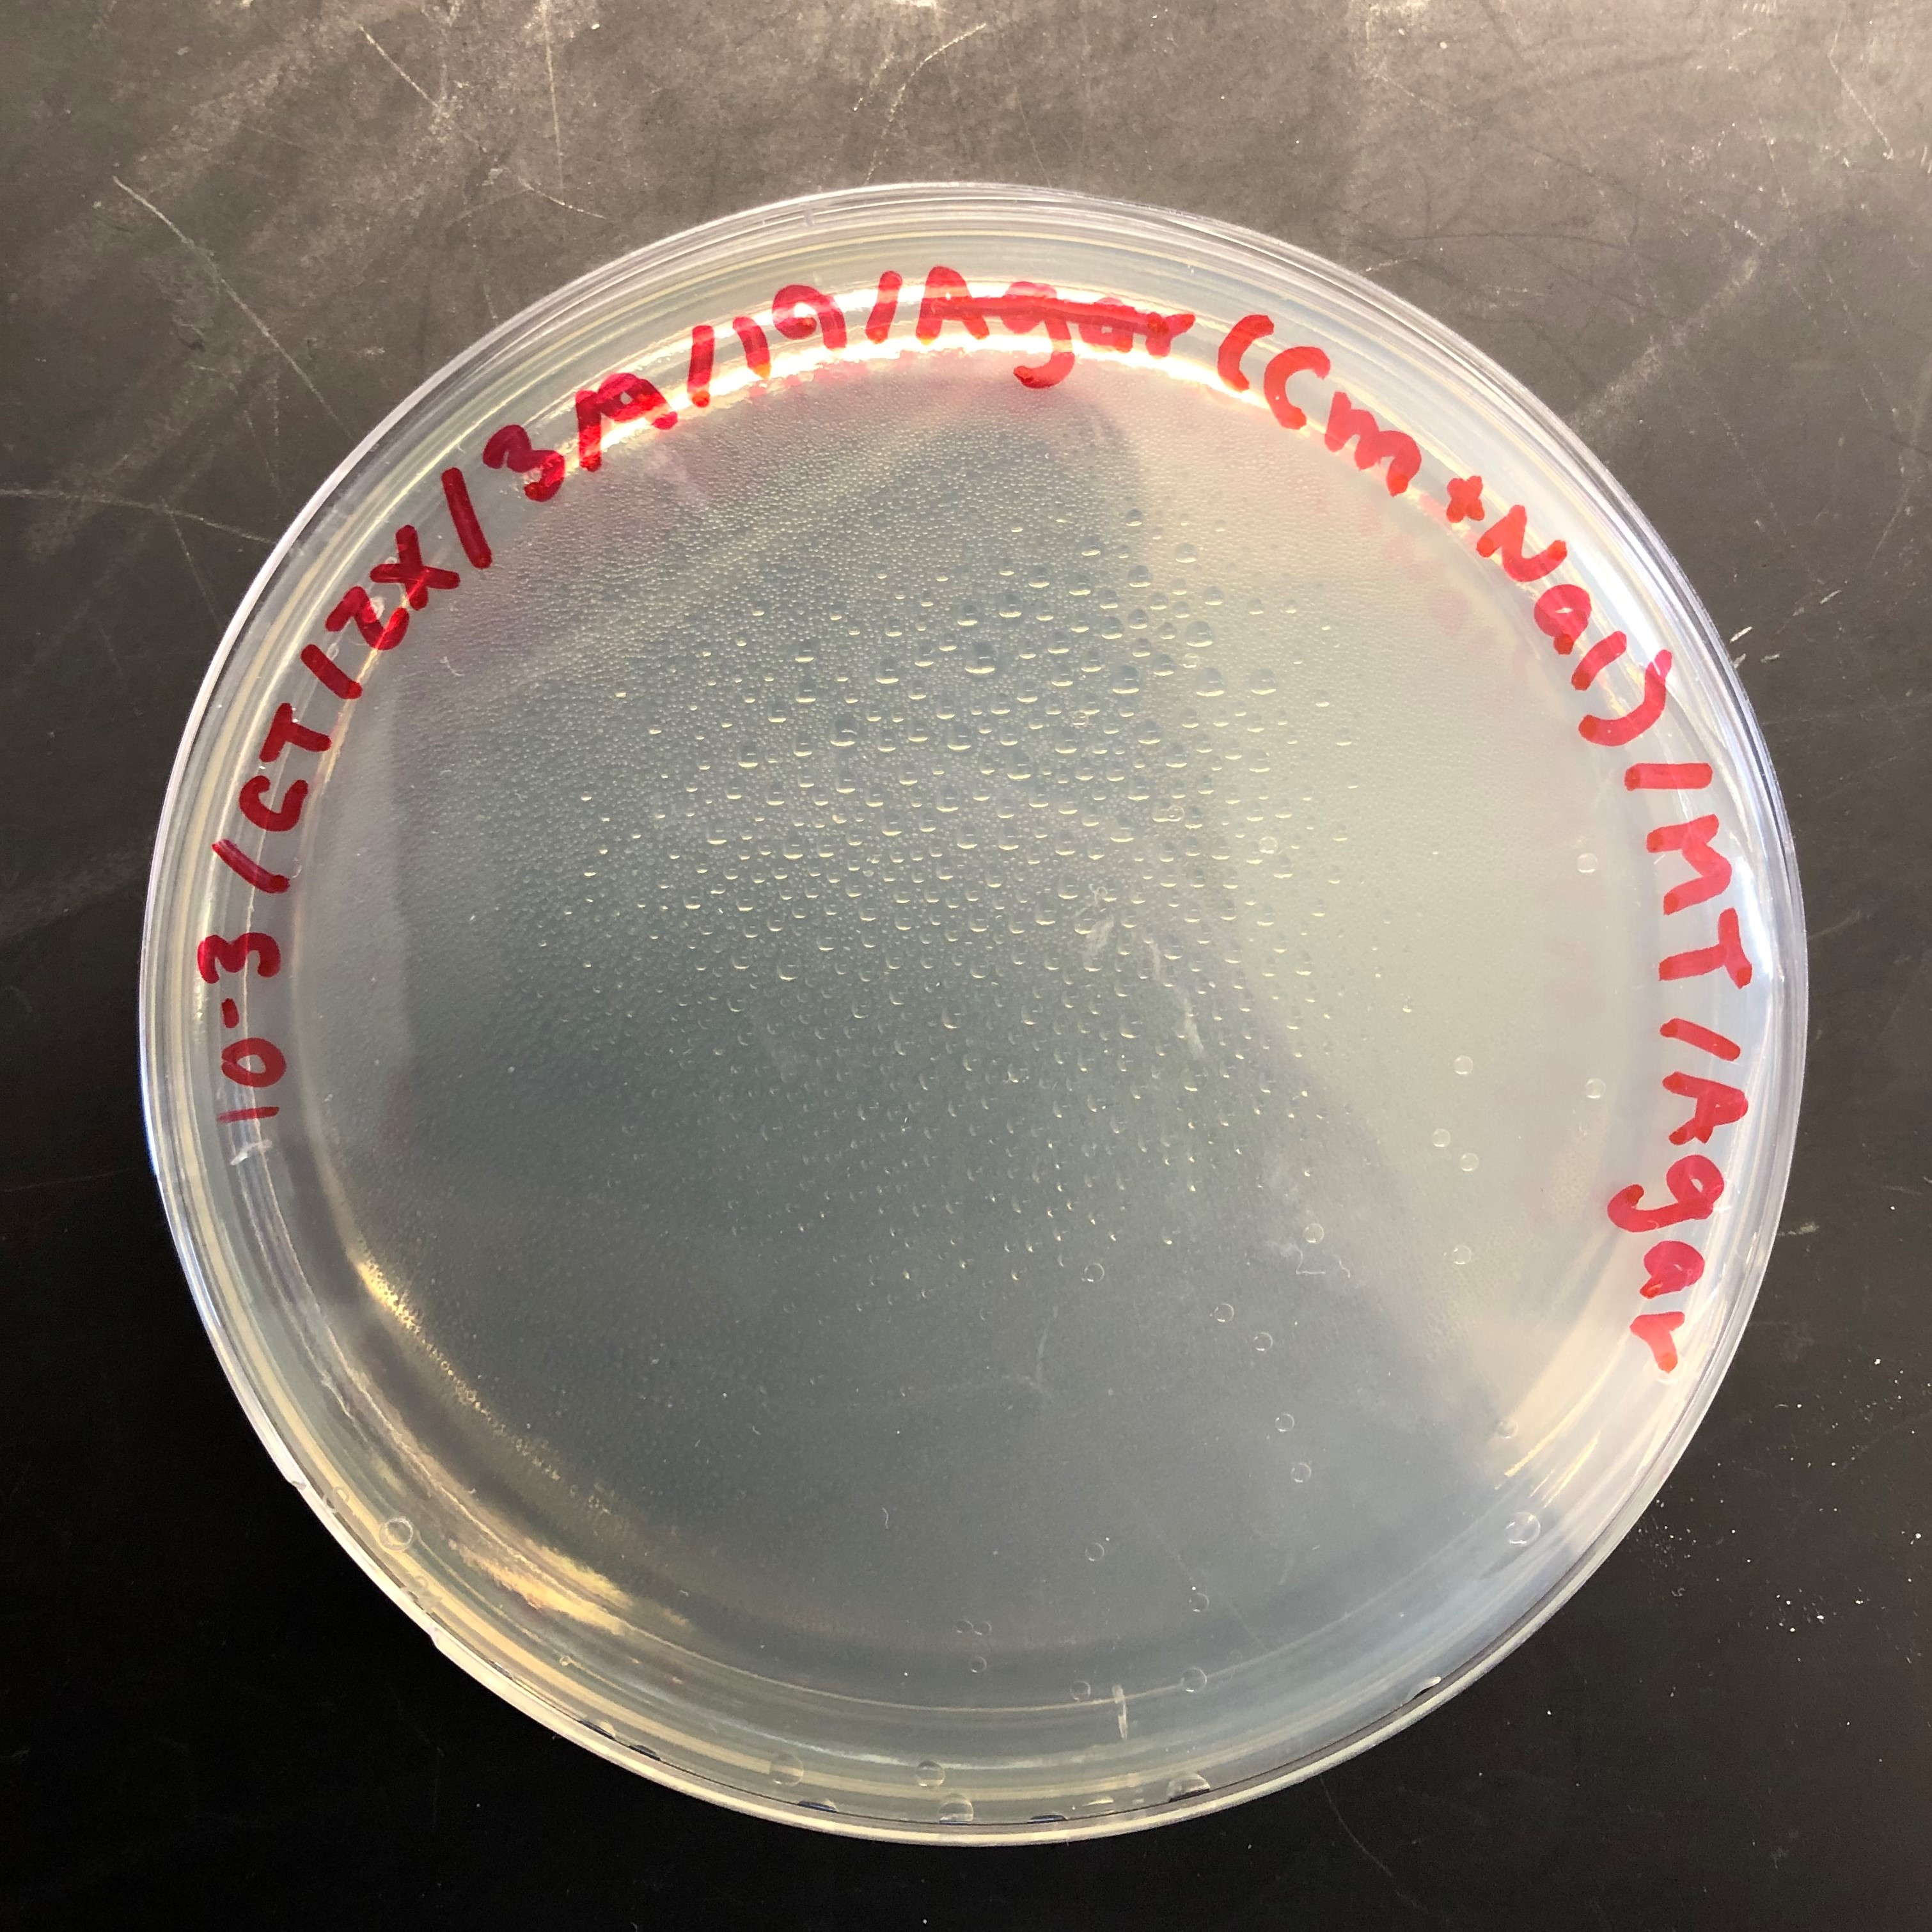
\includegraphics[width = 0.9\linewidth]{Mate_3_NalCm.jpg}
					\captionsetup{font={scriptsize}}\caption{MT $10 ^ {-3}$ Cm-Nal, 0}
				\end{minipage}
			\end{figure}
			\begin{figure}[H]
				\begin{minipage}[t]{0.32\textwidth}
					\centering
					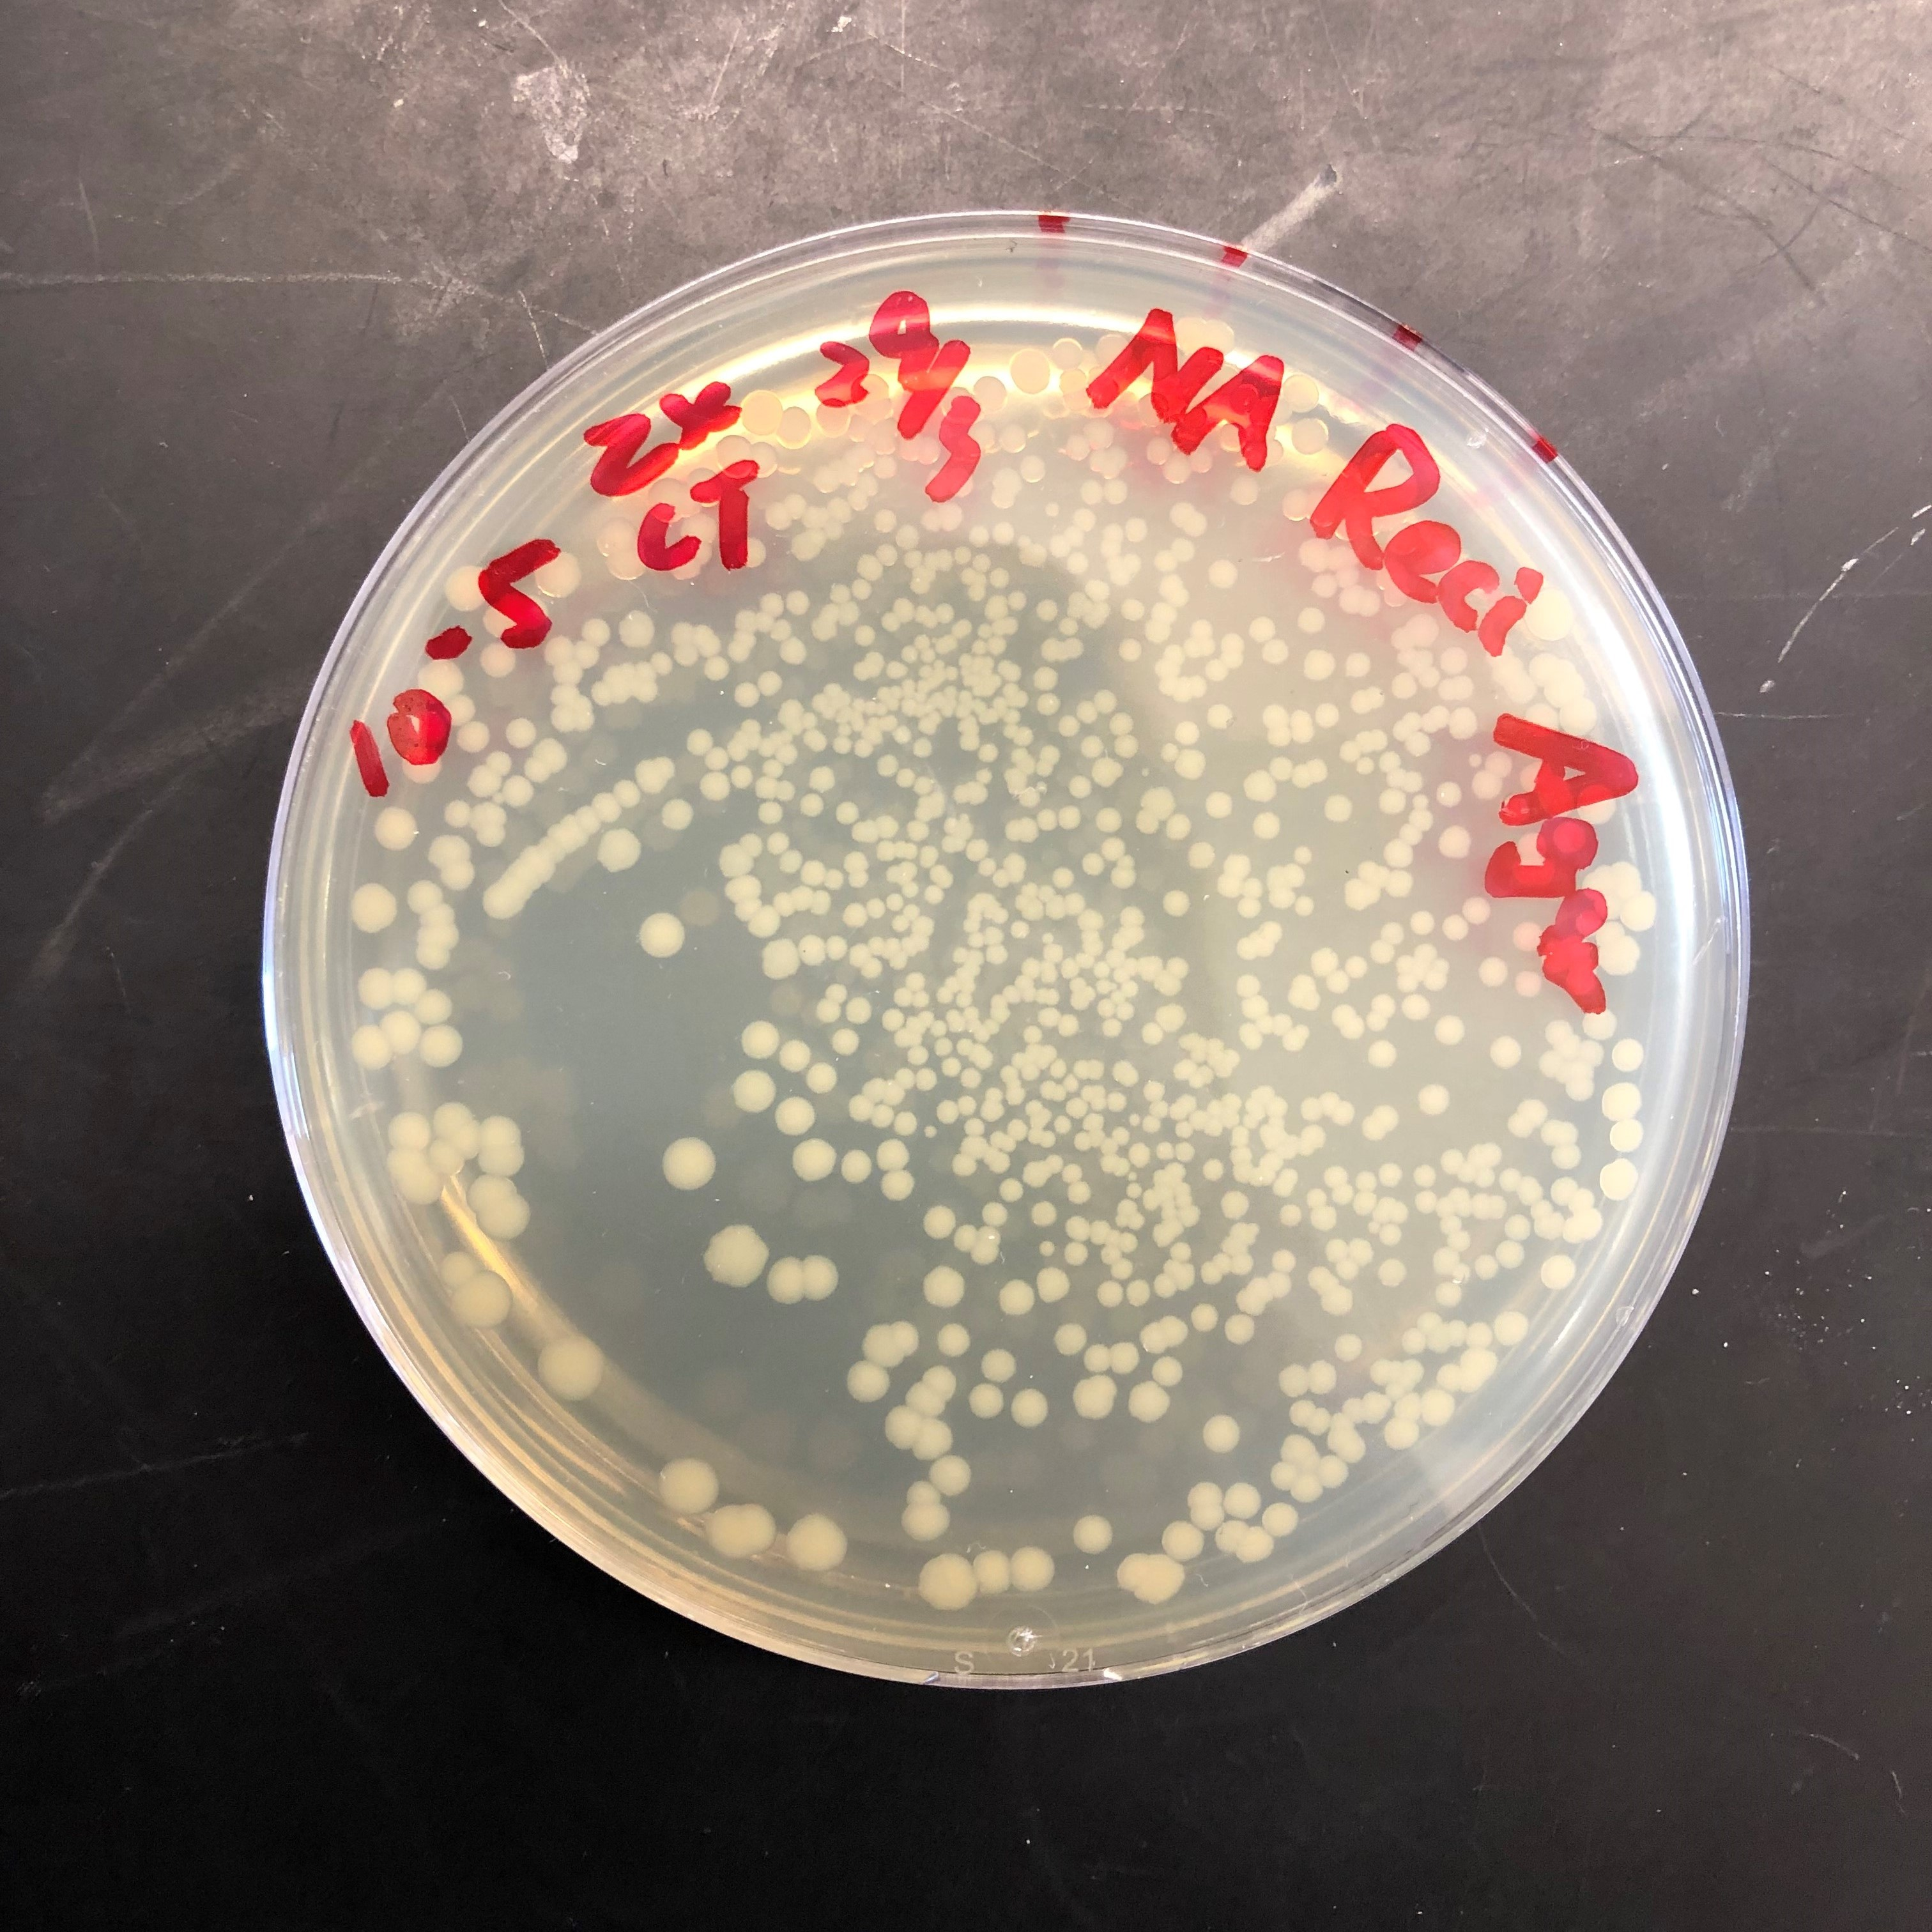
\includegraphics[width = 0.675\linewidth]{Reci_5_NA.jpg}
					\captionsetup{font={scriptsize}}\caption{R $10 ^ {-5} $ NA, 946}
				\end{minipage}
				\begin{minipage}[t]{0.32\textwidth}
					\centering
					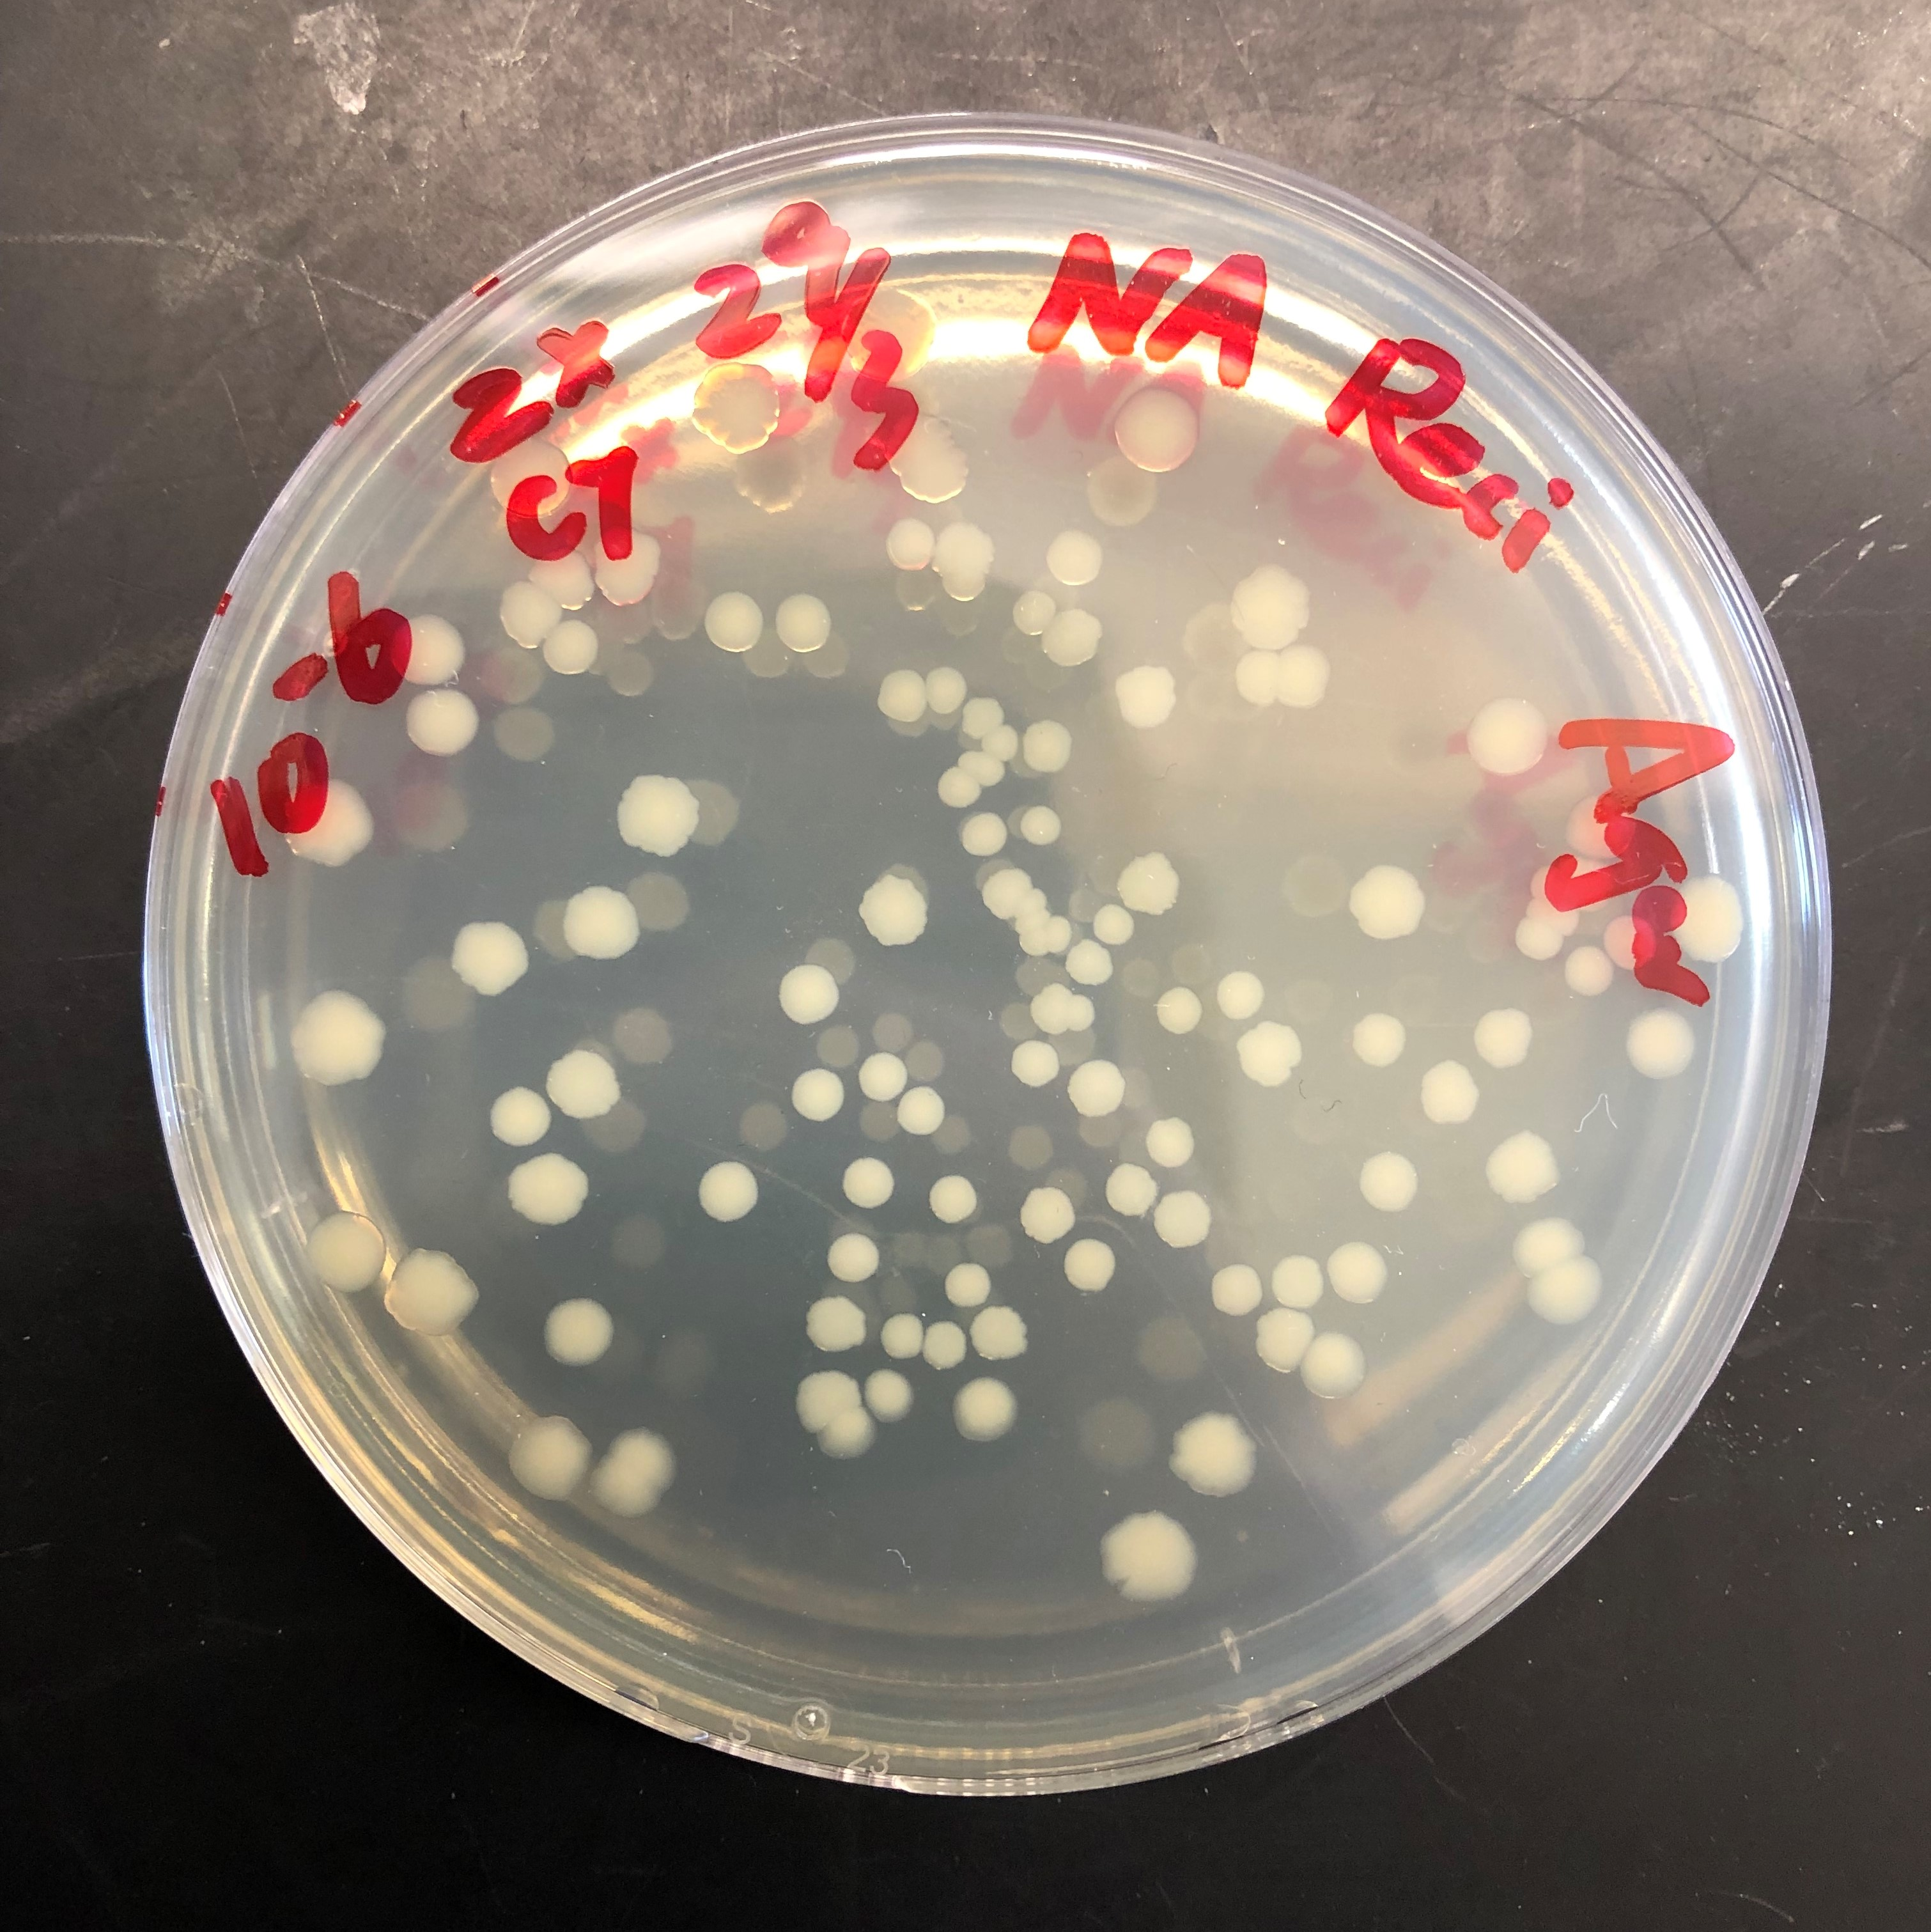
\includegraphics[width = 0.675\linewidth]{Reci_6_NA.jpg}
					\captionsetup{font={scriptsize}}\caption{R $10 ^{-6} $ NA, 107}
				\end{minipage}
				\begin{minipage}[t]{0.32\textwidth}
					\centering
					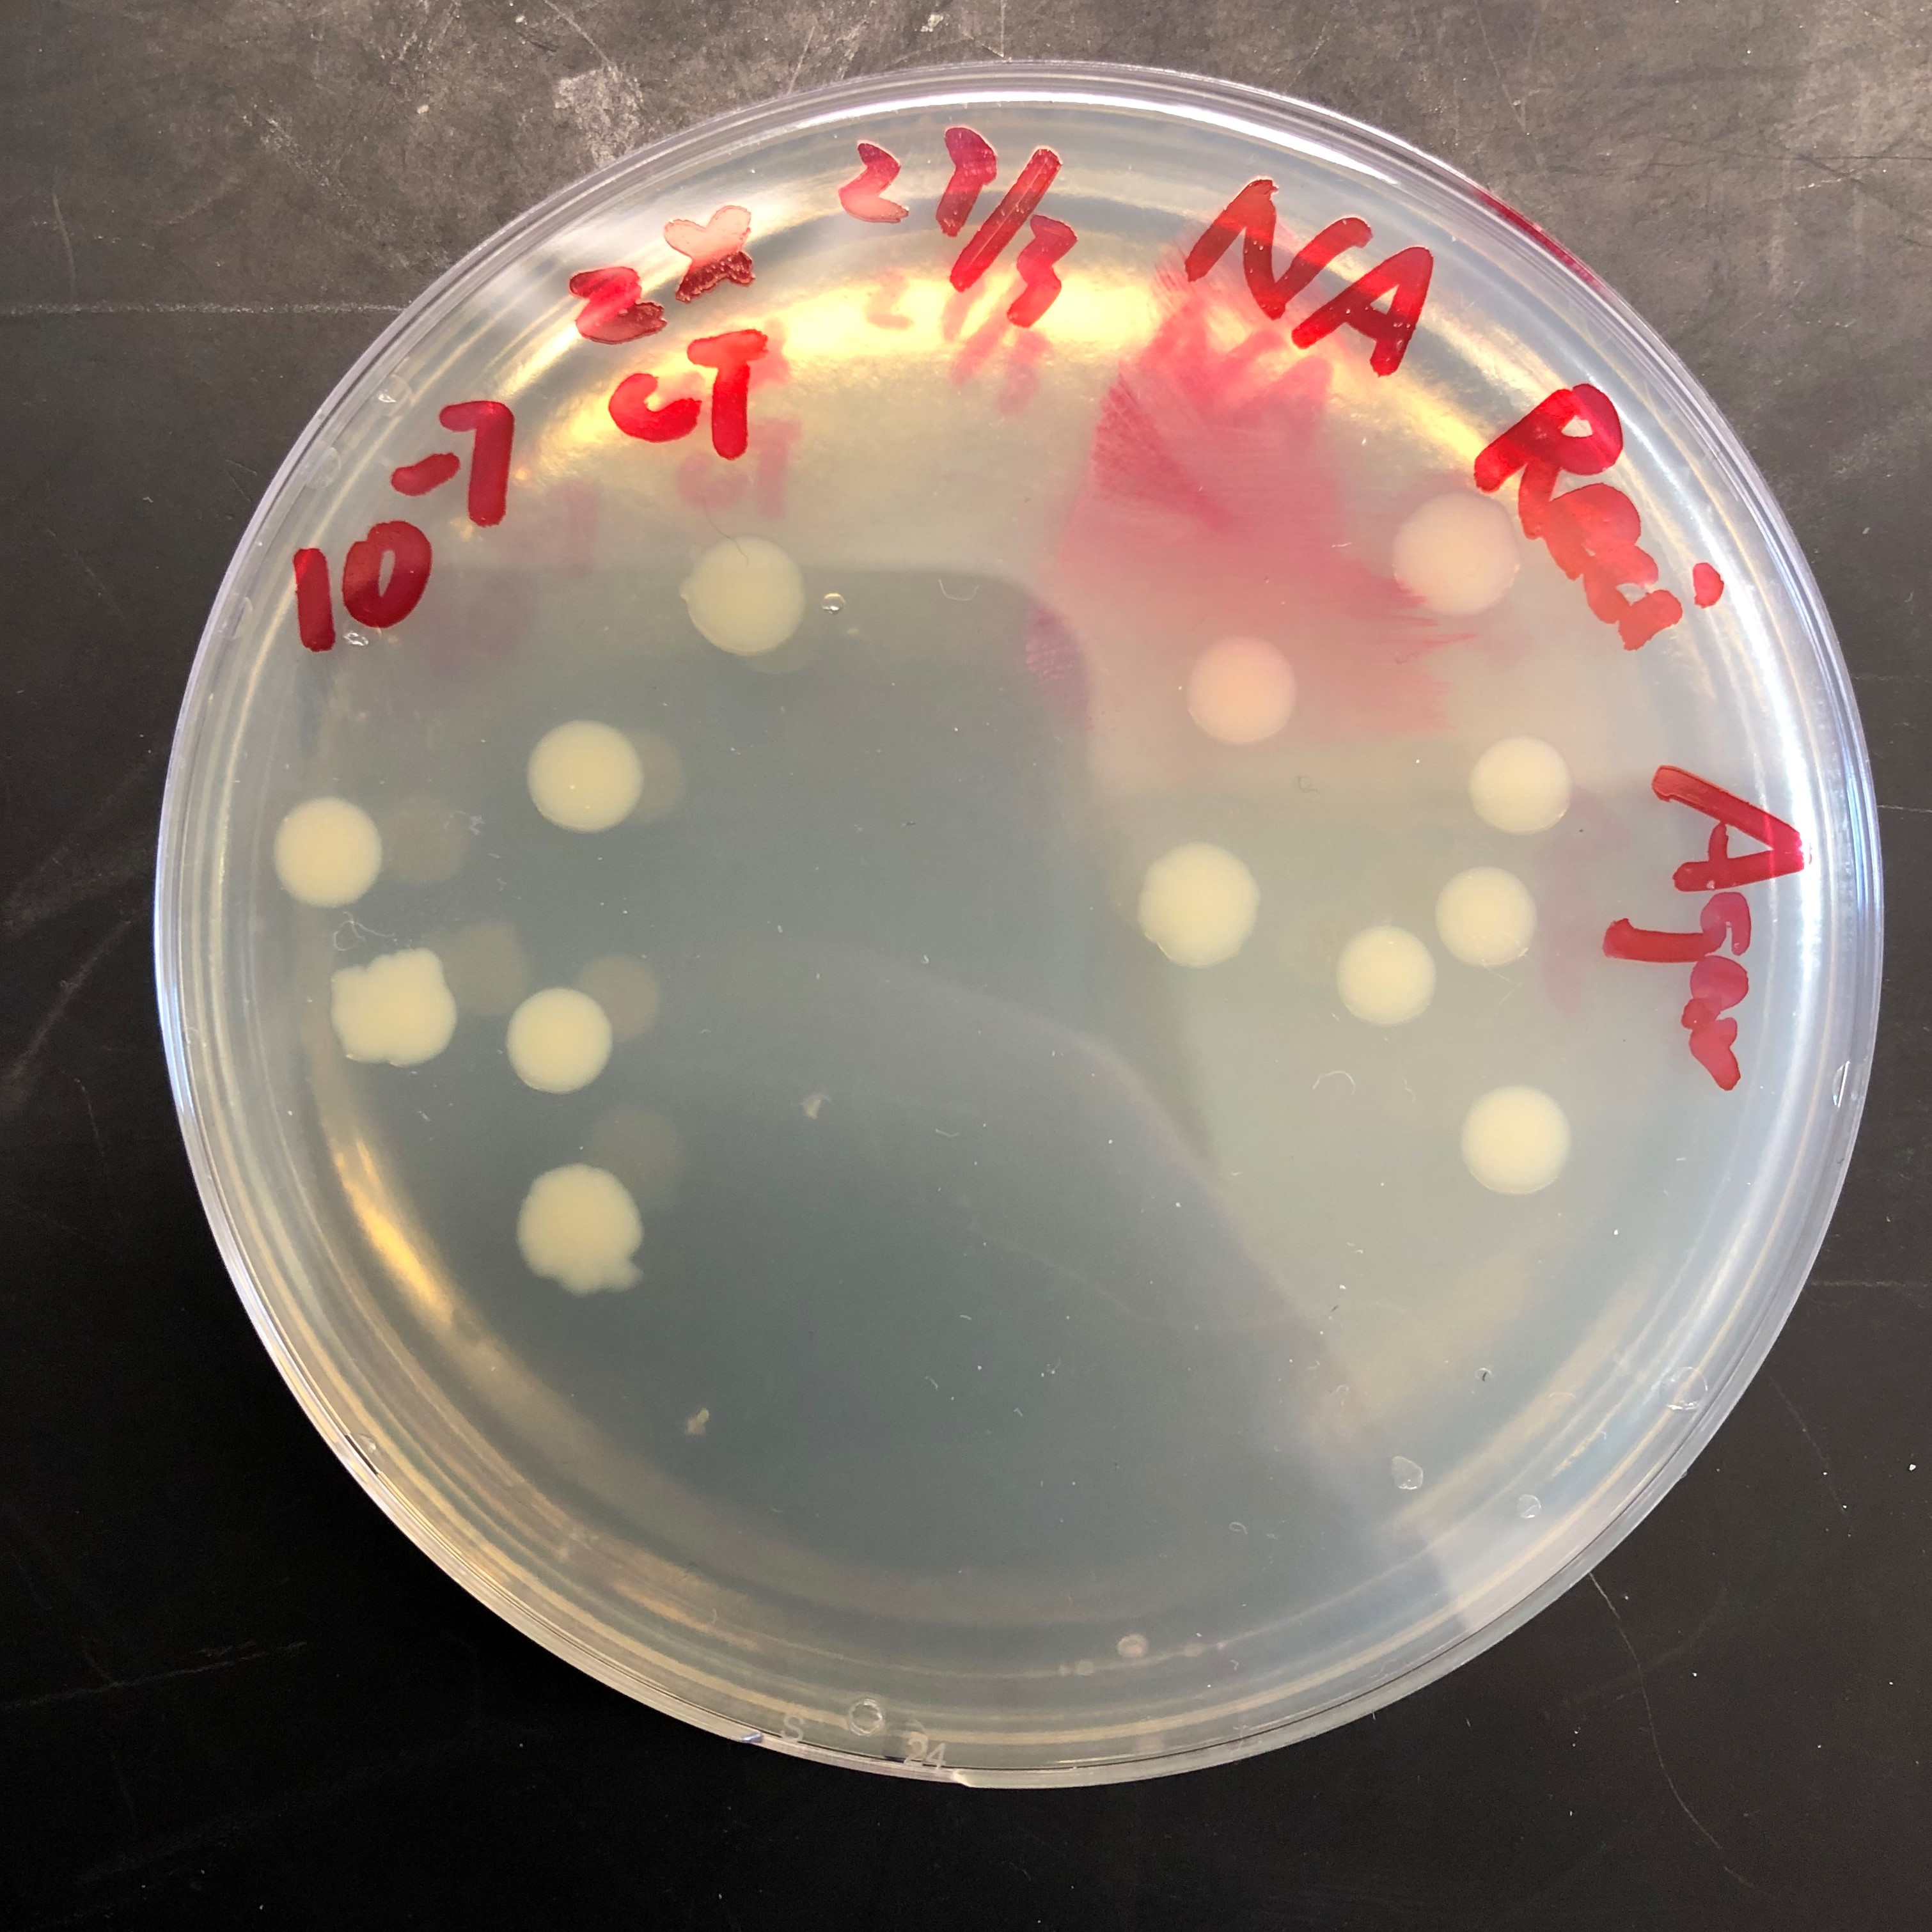
\includegraphics[width = 0.675\linewidth]{Reci_7_NA.jpg}
					\captionsetup{font={scriptsize}}\caption{R $10^{-7}$ NA, 13}
				\end{minipage}
			\end{figure}
			\begin{figure}[H]
				\begin{minipage}[t]{0.5\textwidth}
					\centering
					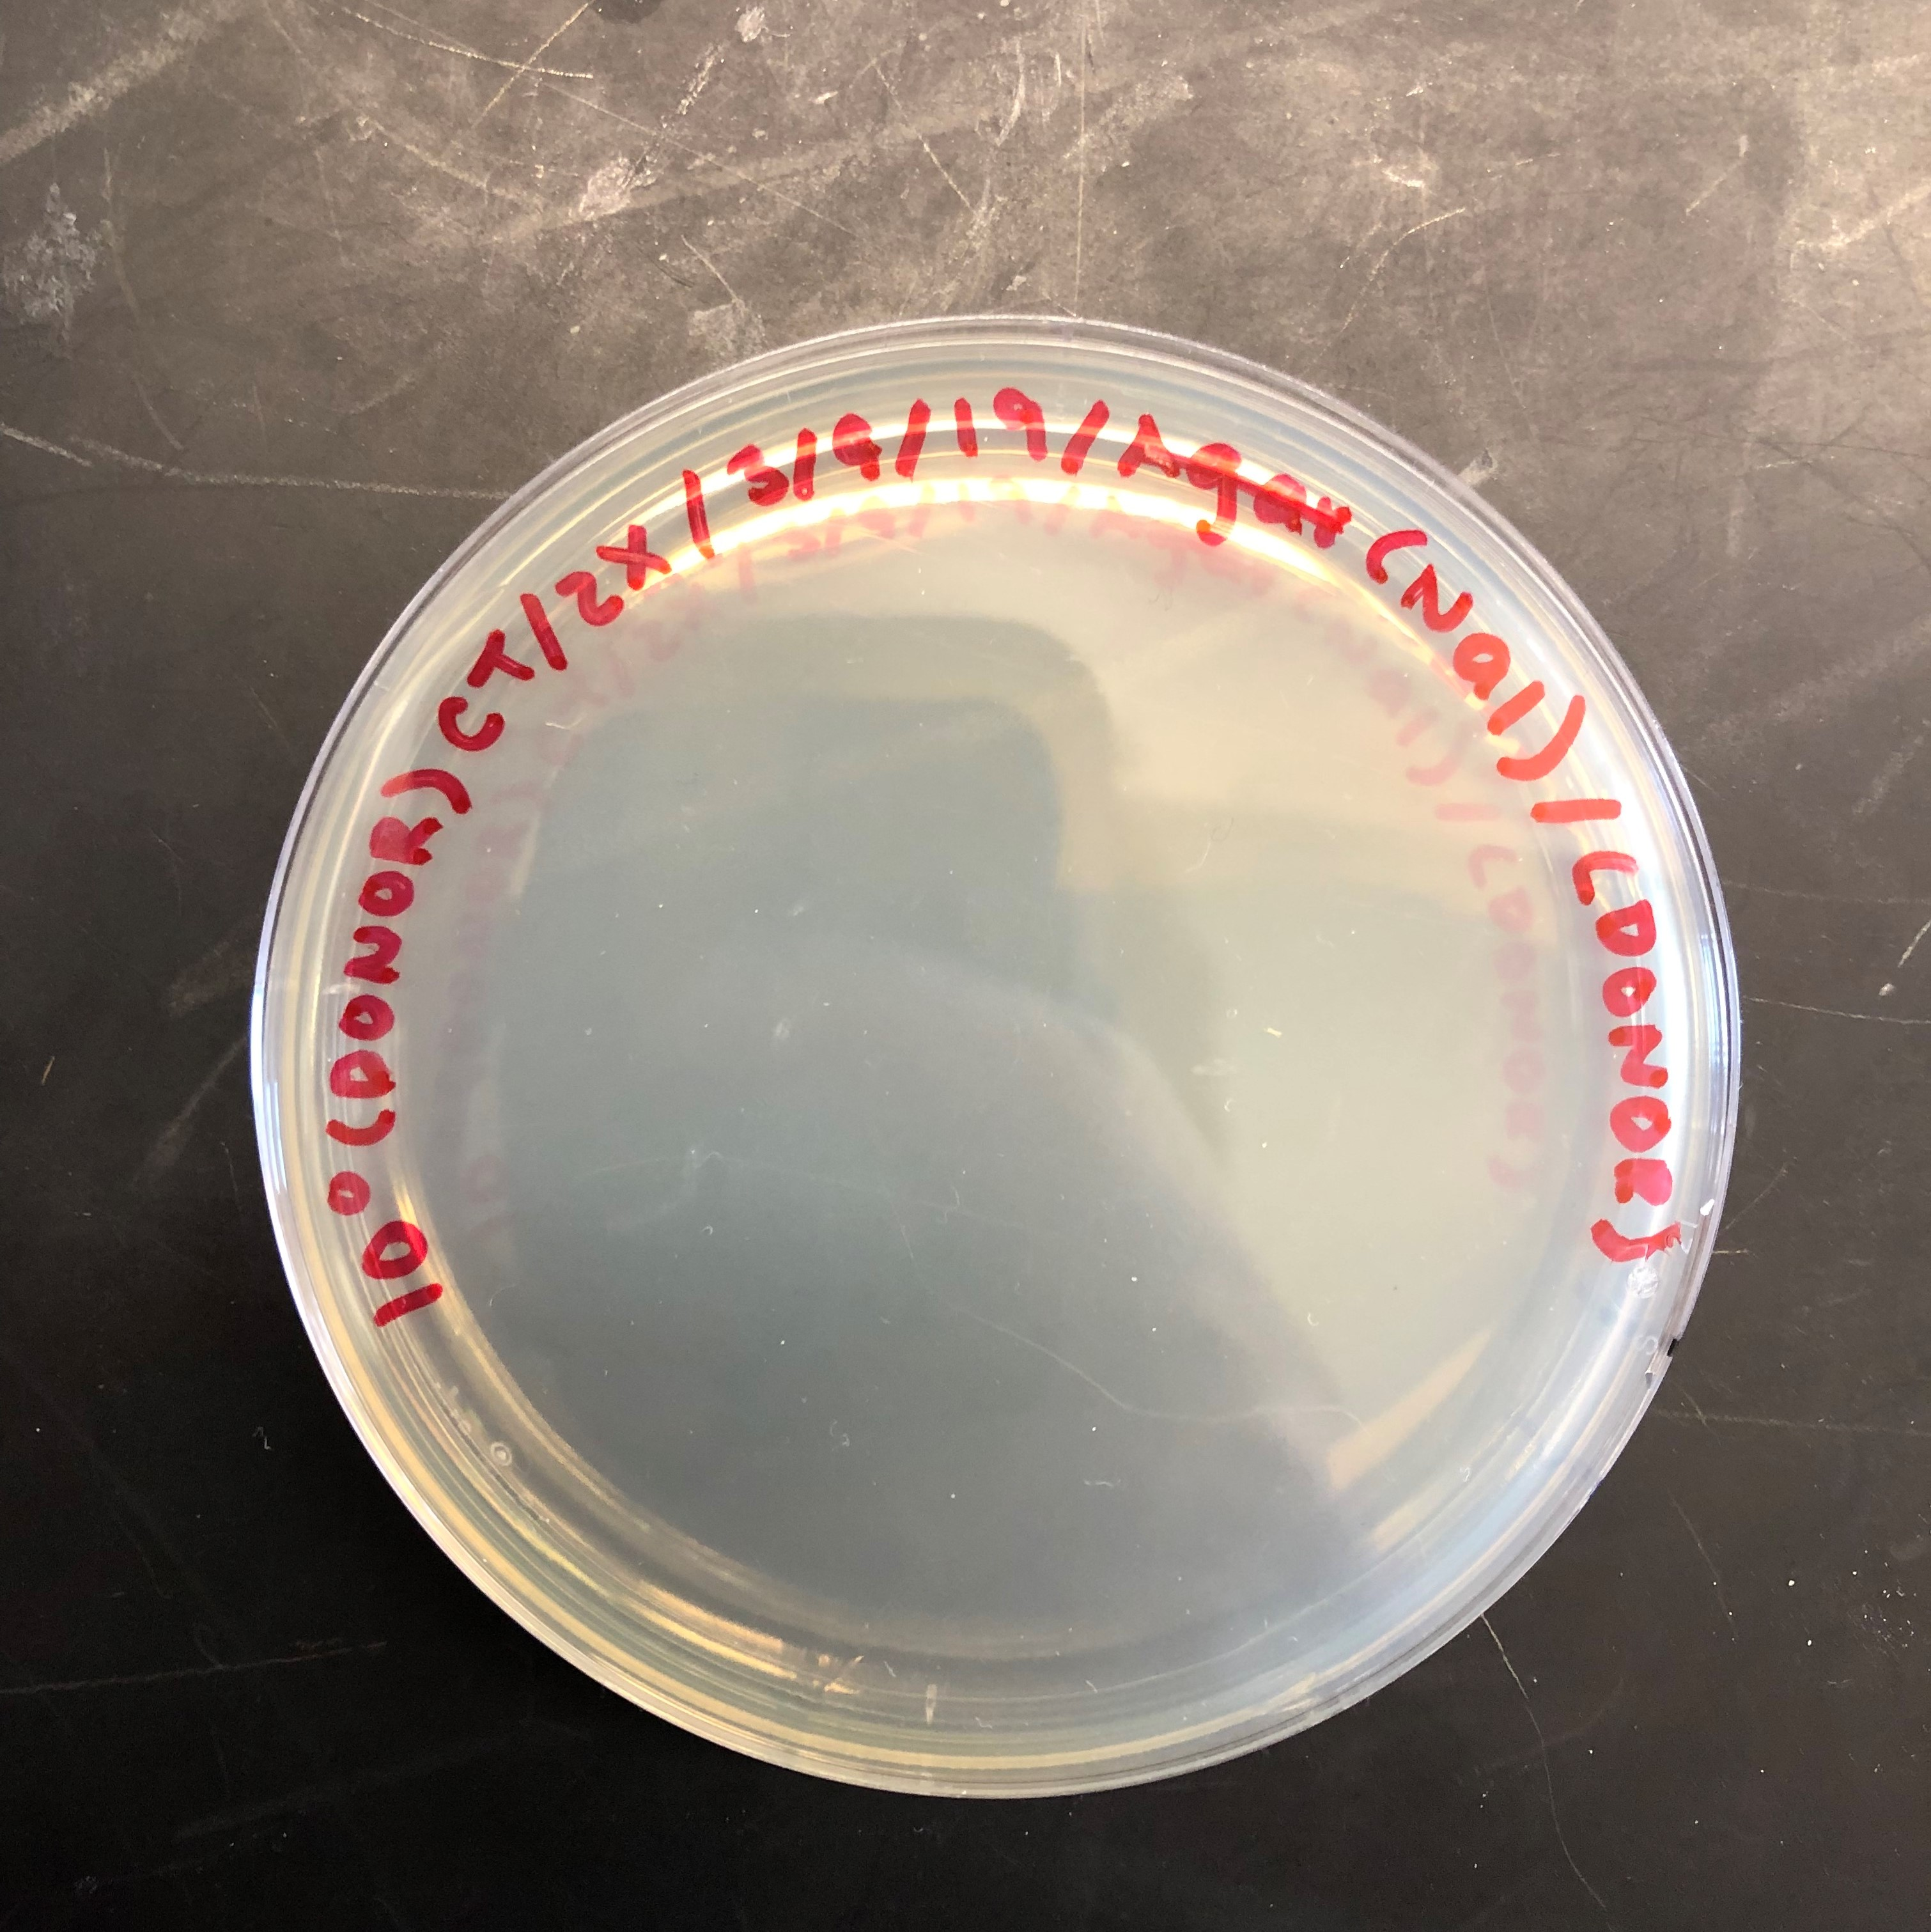
\includegraphics[width = 0.432\linewidth]{Done_0_Nal.jpg}
					\captionsetup{font={scriptsize}}\caption{D $10^0$ Nal, 0}
				\end{minipage}
				\begin{minipage}[t]{0.5\textwidth}
					\centering
					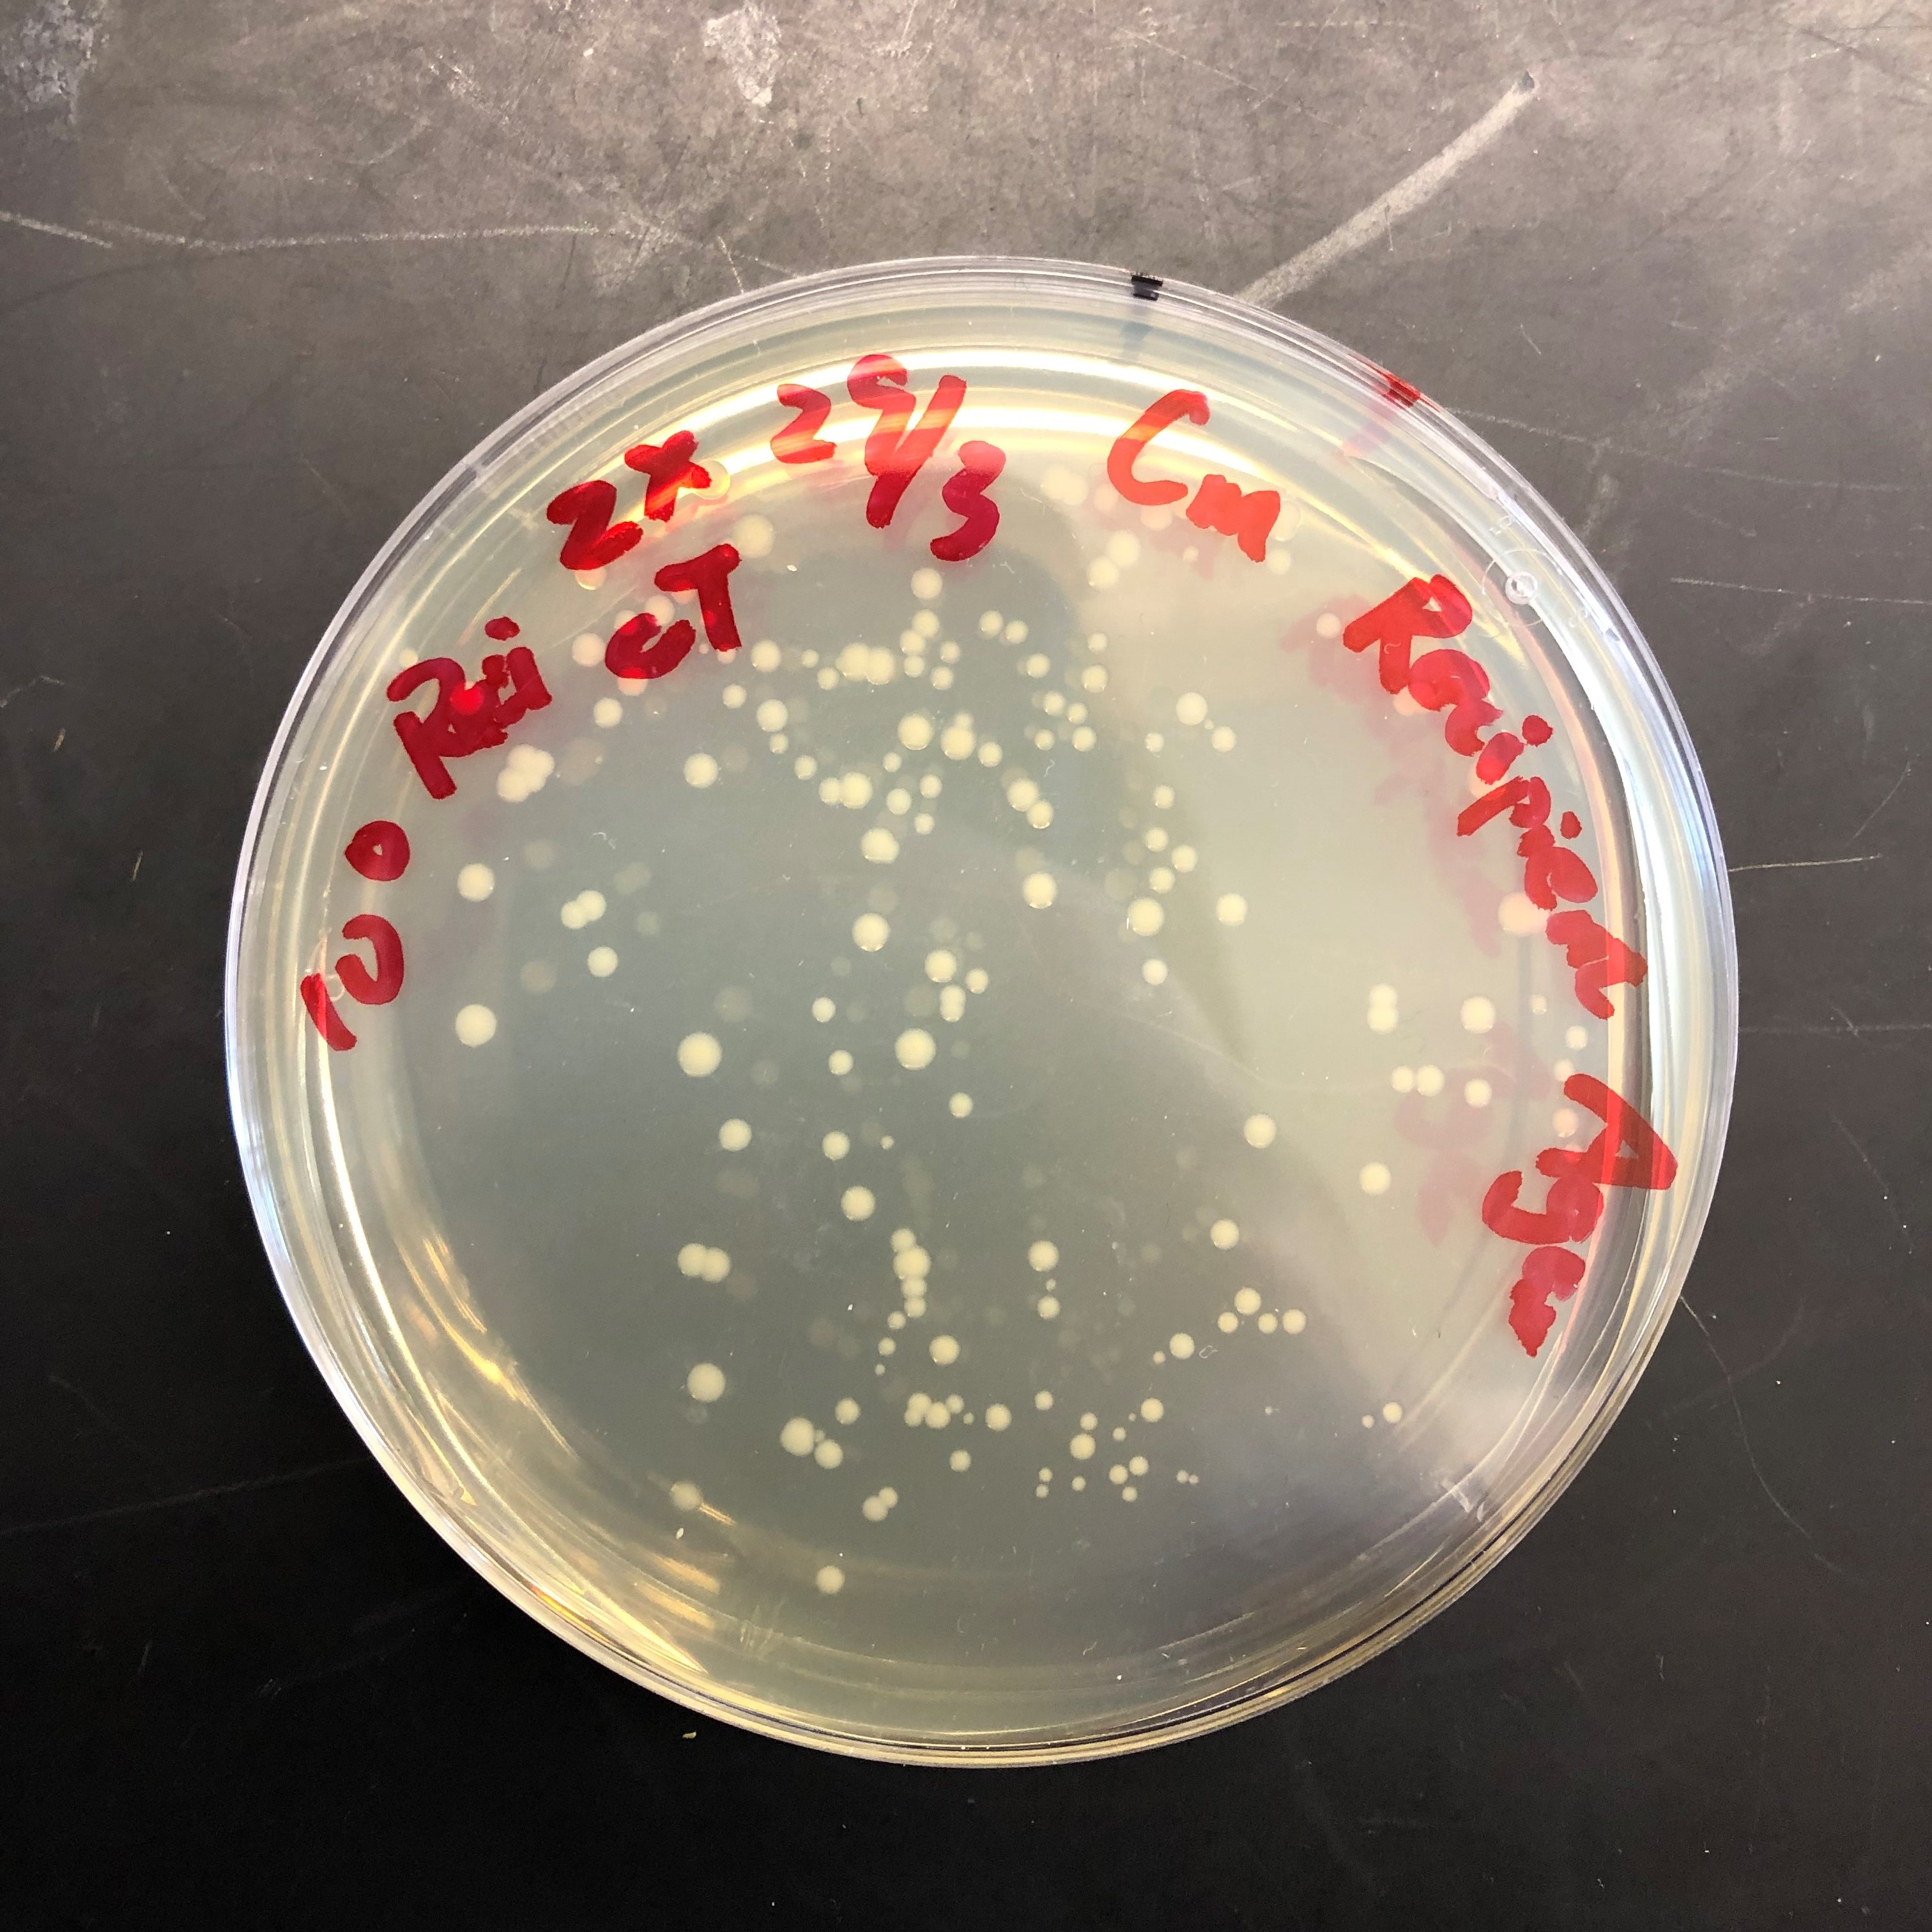
\includegraphics[width = 0.432\linewidth]{Reci_0_Cm.jpg}
					\captionsetup{font={scriptsize}}\caption{R $10 ^ 0$ Cm, 135}
				\end{minipage}
			\end{figure}
			\subsubsection{General Description} 
			The colonies are white and round. The size of colonies varies at the plates with $10 ^ 0$ dilution. This phenomenon indicates that if the plate starts with higher concentration of cells, the colonies are more likely to start from several cells instead of one single cell, which makes the size of colonies different.

			\subsubsection{Percent Conjugation Calculation} 
			\paragraph{Number of Conjugation} There are three kinds of cells that can survive on Cm-Nal plates, the cells after conjugation, the mutant of recipient that is insensitive to Cm, and the mutant of donor that is insensitive to Nal. So the total number of successful conjugation is as follows. Here, I discarded the other three numbers of Cm-Nal plates, since they are too small (2 in $10 ^ {-1}$, 0 in $10^{-2}$, 0 in $10 ^ {-3}$), probably because of the wrong operation in experiment.
			$$
			\begin{aligned}
			\#\text{Conjugation} &= \#\text{Colonies.of.Cm.Nal} - \#\text{Recipient.Mutant} - \#\text{Donor.Mutant}\\
			&= 508 - 135 - 0\\
			&= 373
			\end{aligned}
			$$

			\paragraph{Explanation to Control Plates} Ideally, there if no mutations or contamination happened to recipient and donor cells, they should not survival on Cm plates and Nal plates, respectively. However, in Cm plates of recipient cells, there are 135 colonies. One explanation is that the mutation happened to recipient cells. The second explanation is contamination. Because of their similar shape, color, and size, I do not consider these colonies as contamination of environmental microorganism. but it can be contaminated by donor cells due to shared tips.

			\paragraph{Total Number of Recipient Cells} This is calculated by the average of three recipient NA plates, and times the dilution $10 ^ {5}$.
			$$
			\begin{aligned}
			\#\text{Total.Recipient} &= \frac{946 + 107 \times 10 + 13 \times 100}{3} \times 10 ^{5}\\
			&= 1.105 \times 10 ^ 8
			\end{aligned}
			$$ 
			
			\paragraph{Percent Conjugation} This equals to conjugation number divided by total number.
			$$
			\begin{aligned}
			\text{conjugation}\% &= \frac{373}{1.105 \times 10 ^ 8}\times 100 \%\\
			&\approx 3.4 \times 10 ^ {-4}\%
			\end{aligned}
			$$

			\paragraph{Summary} The percentage indicates that conjugation is a rare occurrence. In my opinion, this might be because the concentration of cells is not so high, causing recipient cell and donor cell cannot contact with each other easily. Moreover, this also might be because conjugation is an energy-consuming behavior, and it is used to recombine genes to deal with extreme environment. So if the environment is suitable for cells, they might be less likely to conjugate with others, instead, they will only multiply themselves.
		\subsection{Transposition}
			\begin{figure}[H]
				\foreach \t in {0,...,3}{
					\ifthenelse{\t=0}{\newcommand{\num}{-/-}}{
					\ifthenelse{\t=1}{\newcommand{\num}{3W/8654B}}{
					\ifthenelse{\t=2}{\newcommand{\num}{0W/728B}}{
					\ifthenelse{\t=3}{\newcommand{\num}{0W/94B}}{}}}}
					\begin{minipage}[t]{0.23\textwidth}
						\centering
						\includegraphics[width = 0.9\linewidth]{Tran_\t_Xgel.jpg}
						\captionsetup{font = {scriptsize}}
						\caption{IT $10 ^ {-\t}$ Xgel-Kan, \num}
					\end{minipage}
				}
			\end{figure}
			\begin{figure}[H]
				\foreach \t in {4,...,7}{
					\ifthenelse{\t=4}{\newcommand{\num}{-}}{
					\ifthenelse{\t=5}{\newcommand{\num}{820}}{
					\ifthenelse{\t=6}{\newcommand{\num}{103}}{
					\ifthenelse{\t=7}{\newcommand{\num}{12}}{}}}}
					\begin{minipage}[t]{0.23\textwidth}
						\centering
						\includegraphics[width = 0.9\linewidth]{Tran_\t_NA.jpg}
						\captionsetup{font = {scriptsize}}
						\caption{IT $10 ^ {-\t}$ NA, \num}
					\end{minipage}
				}
			\end{figure}
			\subsubsection{General Description}
			On Xgel-Kan plates, most of the colonies are blue, and only a few of them are white. The white colonies indicates that the transposition happens at the \emph{lacZ} gene. On NA plates, all of them are white.

			\subsubsection{Detail of Blue Colonies}
			Most of the blue colonies are pure blue. Some of them are surrounded by a white ring, making the edge change from dark blue to light blue. This is because when the colonies grow, the transposon $kan^R$ is still in these cells. So after generations, the transposition happens, knocks out the \emph{lacZ} gene, leaving Xgel white.

			\subsubsection{Calculation of Percent Transposition}
			\paragraph{Number of Transposition} After transposition, the cells can survive on Xgel-Kan plates, because the $kan^R$ gene is activated. So the average number of colonies on Xgel-Kan plates are:
			$$
			\begin{aligned}
			\#\text{Transposition} &= \frac{(3 + 8654) + (0 + 725) \times 10 + (0 + 94)\times 100}{3}\\
			&\approx 8445
			\end{aligned}
			$$
			\paragraph{Total Number} The total number of all cells is calculated from the colonies on NA plates, and multipled by the dilution $10 ^ 4$.
			$$
			\begin{aligned}
			\#\text{Total} &= \frac{103 * 10 + 12 * 100}{2} \times 10 ^4\\
			&\approx 1.115 \times 10 ^ 7
			\end{aligned}
			$$
			\paragraph{Percentage of Transposition} The percentage equals to number of transposition divided by total number.
			$$
			\begin{aligned}
			\text{Transposition}\% &= \frac{8445}{1.115 \times 10 ^ 7}\\
			&= 0.076\%
			\end{aligned}
			$$
			\paragraph{Summary} The percentage indicates that transposition is a rare occurrence. The transposon needs transposase to cut the DNA and then starts transposition. The transposase is regulated by lactose operon and IPTG can bind the repressor, so that the promotor can start gene expression and produce transposase. So, the transposition needs many prerequisite and it is not guaranteed that the transposase will transpose $kan^R$ gene. That is why transposition is a rare occurrence.

			\subsubsection{Factors that Interfere Accuracy}
				\begin{enumerate}
					\item Whether $kan^R$ is transposed to a place that has start codon.
					\item Whether $kan^R$ is transposed to a place that has promotor.
					\item Whether $kan^R$ is transposed with right orientation (not reversed).
					\item Whether transposition knocks out the essential gene to cell's life.
				\end{enumerate}

		\subsection{Mutagenesis}
			\subsubsection{Calculation of Percent Mutagenesis}
				The only available data of successful mutagenesis is from Figure 11, where there are 3 white colonies out of 8654 blue ones. Moreover, the average of total number of transposition has been calulated before as 8445 with dilution $10 ^ {-1}$. So the result is:
				$$
				\begin{aligned}
				\text{Mutagenesis}\% &= \frac{\#\text{White}}{\#\text{Total}}\\
				&= \frac{3}{8445} \times 100 \%\\
				&= 0.035\%
				\end{aligned}
				$$
			\subsubsection{Size of \emph{lacZ} Gene}
				If transposition happens at any position with equally probability and there is no other side effect of transposition. Then the size of \emph{lacZ} gene is only 0.035\% of the whole chromosome, which is only a small fraction.
			\subsubsection{Factors that Affect Determination}
				\begin{enumerate}
					\item Whether a white colony started from mutagenesis cell or mutagenesis happened during the growth of a colony.
					\item If the cells had enough functional lactase before mutagenesis, they can use these remaining enzyme to digest X-gel and become blue.
					\item If the transposon is inserted into a essential gene to cell's life, the total number of transposition (denominator) changes.
				\end{enumerate}
	\section{Errors}
		\subsection{Conjugation}
			In Table \ref{conjugation.data}, the first row data does not differ by power of 10, and the number of colonies is too low except the first data. Maybe this is because the wrong experimental operation, which did not carry enough cells between different dilutions. So, I only use the first data.
		\subsection{Transposition}
			Same as the error mentioned above, in Table \ref{transposition.mutagenesis.data}, 820 is far from the 10 times of 103, but the 10 times of 12 is similar with 103. So when calculating the average, I discarded 820, and only used 103 and 12.
		\subsection{Mutagenesis}
			The first column data is empty, because the plates are full of colonies and they are unequally distributed. So it is hard to get the right number of colonies.

	\section{Conclusion}
		All of these three biological processes are very rare during the life of bacteria. It fits the idea of inheritance and mutation in genetics, that the genes pass through generation to generation, and keep unchanged. However, there are still low probability that the gene changes, which brings the new traits or new combinations of old traits. 

		The jumping gene indicates that when the environment is not suitable to the bacteria, they know how to recombine their genes with other individuals to survive, and to adapt the new environment. In some way, this is kind of natural selection. The individuals (or populations) with adaptive genes (or traits) can survive and transfer their genes to their offspring, namely, evolution.

		We can use transposon and transposase to bind a new DNA fragment to bacteria's chromosome, which gives us a new method to change the genotype of a bacteria. 
\end{document}